\documentclass[11pt]{article}

\usepackage[review]{acl}
\usepackage{times}
\usepackage{latexsym}
\usepackage[T1]{fontenc}
\usepackage[utf8]{inputenc}
\usepackage{microtype}
\usepackage{inconsolata}
\usepackage{graphicx}
\usepackage{amsmath,amssymb,amsthm}
\usepackage{booktabs}
\usepackage{xcolor}
\usepackage{array}
\usepackage{tikz}
\usetikzlibrary{arrows.meta,positioning,fit}
\usepackage{pgfplots}
\usepackage{xr}
\externaldocument[M-]{main}
\pgfplotsset{compat=1.16}

\newtheorem{proposition}{Proposition}
\newtheorem{corollary}{Corollary}
\newcommand{\carve}{\textsc{Carve}}
\newcommand{\todo}[1]{\textcolor{red}{[TODO: #1]}}
\DeclareMathOperator*{\argmax}{arg\,max}


\title{Supplementary Appendices for\\``Auditing Verification Decisions in Agent Self-Improvement''}

\author{Anonymous ACL submission}

\renewcommand{\thesection}{S\arabic{section}}
\renewcommand{\thetable}{S\arabic{table}}
\renewcommand{\thefigure}{S\arabic{figure}}
\renewcommand{\theequation}{S\arabic{equation}}
\begin{document}
\maketitle

These appendices accompany the paper. Section, table, figure and equation numbers without the prefix S refer to the paper; Appendices A--E of the paper repeat the terms of Appendix~\ref{app:guide}, a summary of Appendix~\ref{app:rrsi}, selected tables and Appendices~\ref{app:repro} and~\ref{app:claims}.


\section{Guide to the Appendices}
\label{app:guide}
Appendices~\ref{sec:study1}--\ref{app:shopdesk} cover Study 1: its setup and results, the accounting framework, measurements and net values, the verification policies on the intervention banks and their robustness, judges, the harm model, held-out ablations and ShopDesk. Appendices~\ref{app:rrsi}--\ref{app:bk} cover Study 2: the RRSI port and registrations, the first trajectory, AppWorld, margins and decision rules, the validation of the stopping rule (calibration, the cost-aware rule, simpler savings, other noise bands, an acceptance rule without the cost and novelty branch, and savings spent on more rounds), where the reference gains and what dropped acceptances were worth, the independent loops and BK. Appendix~\ref{app:repro} lists the released materials, Appendix~\ref{app:claims} sorts the conclusions by the evidence behind them, and Appendix~\ref{app:carve} describes the multi-fidelity policy and its simulator. The terms used throughout are defined below.

\subsection*{Terms and Abbreviations}
\phantomsection\label{app:terms}

\begin{description}\itemsep0pt
\item[Harness, change, candidate.] The prompts, tool descriptions and code around the frozen agent model; a proposed edit to it; a change the loop measures.
\item[Incumbent.] The harness a round's candidates are proposed against.
\item[Deployment gain, transfer.] A candidate's held-out success minus its incumbent's; a loop's held-out success after round 9 minus that of the base harness.
\item[Evolve and held-out tasks.] $\tau^2$'s training split, on which the loop evaluates candidates, and its test split, on which we deploy them.
\item[Full evaluation.] RRSI's selection: every candidate is run twice on every evolve task.
\item[Noise band $\delta$.] RRSI's threshold, calibrated from three evaluations of the base harness. A candidate above it is admitted if its cost change is within budget; inside it (the \emph{in-band branch}), if a score of its success change, cost change and novelty is positive.
\item[Sequential full evaluation (registered rule).] Full evaluation run in batches of 10 that stops a candidate once the predicted probability that RRSI's rule admits it falls below $\gamma=0.05$, with the cost change held at its running estimate.
\item[Cost-aware rule.] The same, with the uncertainty of the final cost change modelled (Appendix~\ref{app:r9}).
\item[Admission, history.] Which candidates a rule can accept; the scores of evaluated candidates that RRSI shows the proposer in later rounds.
\item[Decision value $D$.] The held-out gain of a rule's choice, averaged over rounds, zero when it keeps the incumbent.
\item[Agreement, recall.] The share of rounds in which a rule makes full evaluation's choice; the share of full evaluation's acceptances it makes.
\item[r1--r4, E3.] Recorded trajectories of RRSI driven by full evaluation on $\tau^2$ (r4 with a thinking proposer) and on AppWorld.
\item[CL, IL, BK.] Loops driven by sequential evaluation (two, descriptive); the registered comparison of six independent loops per rule; the registered blocked comparison of five rules in four blocks that share one calibration (Appendix~\ref{app:bk}).
\item[Episode, episode equivalent.] One run of the agent on a task; the token cost of a replay or check relative to an episode.
\end{description}

\section{Study 1: One Round of Attribution-Driven Repair}
\label{sec:study1}

\paragraph{Setup.} A DeepSeek-V4-Flash agent, with the provider's default sampling, works on the retail and airline domains of $\tau^2$-bench \citep{yao2024taubench,barres2025tau2}, mostly on injected faults; DeepSeek-V4-Pro attributes failures \citep{wan2024tntllm}, writes patches and judges. For 36 (category, component) cells per domain the analyst writes three patches, each with 20 targeted replays, single-step checks and 4 to 20 regression runs, plus 20 null replays per category. Eleven policies spend a budget from these \emph{intervention banks}: \emph{Apply attributed} applies the most-blamed components' first patches unverified, and the others use replays, regression gates in the style of HarnessFix \citep{chen2026harnessfix}, uncertainty sampling or multi-fidelity allocation (\carve{}, Appendix~\ref{app:carve}). Budget-10 sets are deployed on 40 retail and 20 airline unseen tasks, 3 episodes each; retail was the development domain (Appendices~\ref{app:s1tables} and~\ref{app:shopdesk}).

\paragraph{Results: too little resolution.} Unverified attributed patches raised held-out success by 11.7 points on retail [$4.5,18.8$] and 6.7 on airline [$-3.3,16.6$] (Table~\ref{tab:deploy}). No verified set reliably improved over them ($-4.3$ to $+0.3$ and $-4.0$ to $-0.3$ points, with intervals reaching $+6.0$ and $+8.5$, so not equivalence; one, the HarnessFix-style bundle gate, was worse on retail, $-2.7$ [$-5.0,-0.4$], unadjusted for the comparisons): the sets' replay-predicted gains differed by 1.0--1.7 points, below 2.6--3.8 points of deployment noise, and 20--23\% of unpatched replays succeed anyway (Table~\ref{tab:measured}). One round of text patches cannot resolve whether verification selects better changes (Table~\ref{tab:netn}), and does not show that it brings no benefit; Study 2 therefore uses many rounds of code edits and deploys every candidate.



\section{An Accounting Framework for Single-Round Repair}
\label{app:framework}

\paragraph{Setting.} An agent is assembled from \emph{components} $j$ (prompt sections, tool descriptions, configuration). On a task distribution it fails with rate $F$; an LLM groups its failures into categories $i$ with shares $f_i$. For each \emph{cell} $(i,j)$ that the analyst blames, it proposes $K$ candidate patches $k$ that rewrite component $j$. Let $e_{ij}\in\{0,1\}$ indicate whether changing $j$ can repair category $i$ at all, and $q_k$ the fraction of category-$i$ failures that patch $k$ repairs if so. Separating $e$ from $q$ matters because a patch that fails to help may be aimed at the wrong component or merely be a bad patch. We call a cell with $e_{ij}=1$ an \emph{effective edge}. This is an interventional notion: some change to $j$ repairs failures of category $i$. It need not mean that $j$ was the original cause of those failures.

\paragraph{Net effect.} Applying patch $k$ of cell $(i,j)$ changes the success rate by
\begin{equation}
\Delta_k = F f_i e_{ij} q_k - (1-F)\rho_k - c_{\mathrm{a}} - c_{\mathrm{w}}(1-e_{ij}),
\label{eq:delta}
\end{equation}
where $\rho_k$ is the patch's absolute excess failure rate on tasks that used to succeed (regressions, which may hit any category): such a task fails a re-run with probability $r_0$ unpatched and $r_0+\rho_k$ patched, so $\rho_k<0$ is possible; $c_{\mathrm a}\ge0$ is a cost charged for every applied change (review, maintenance) and $c_{\mathrm w}\ge0$ a penalty charged only for a change aimed at a wrong component (risk not captured by $\rho_k$). Costs are fractions of the failure mass $F$. The goal is to choose a set of patches, at most one per cell, that maximises $\sum_k\Delta_k$ on held-out tasks; effects of patches to different components are treated as additive, and held-out success of whole patch sets (Table~\ref{tab:deploy}) and a leave-one-out ablation (Appendix~\ref{app:ablate}) are the only checks. A targeted replay of a category-$i$ failure with patch $k$ succeeds with probability $b_i+(1-b_i)e_{ij}q_k$, a null replay with probability $b_i$, and a regression run fails with probability $r_0+\rho_k$.

\paragraph{Value of verification.} Before any evidence, the net effects $\Delta=(\Delta_k)$ of the candidate patches are uncertain, with a prior that reflects the analyst's accuracy and what is known about patch quality and regressions. The \emph{default} applies, in each cell, the patch with the largest $\mathbb E[\Delta_k]$ if that is positive. Verification observes outcomes $Y$ and then chooses; its value is $V(Y)=\mathbb E\big[\max_S\mathbb E[\sum_{k\in S}\Delta_k\mid Y]\big]-\max_S\mathbb E[\sum_{k\in S}\Delta_k]$, before the cost of the experiments. Write $x^+=\max(x,0)$ and $x^-=\max(-x,0)$.

\begin{proposition}[Value of verification]
\label{prop:vpi}
For any experiments $Y$, $V(Y)$ is at most the value of learning $\Delta$ exactly, which is the sum over cells of
\begin{equation}
V_{ij}=\mathbb E\big[\max_k\Delta_k^+\big]-\max_k\big(\mathbb E\Delta_k\big)^+ .
\end{equation}
With $k^\star$ the default patch of the cell,
\begin{equation}
V_{ij}\;\le\;\underbrace{\mathbb E\big[\max_k\Delta_k^+-\Delta_{k^\star}^+\big]}_{\text{choosing among patches}}\;+\;\underbrace{\mathbb E\big[\Delta_{k^\star}^-\big]}_{\text{avoiding harm}},
\label{eq:vpi}
\end{equation}
with equality when the default applies $k^\star$, and $\mathbb E[\Delta_{k^\star}^-]\le(1-F)\,\mathbb E[\rho_{k^\star}^+]+c_{\mathrm a}+c_{\mathrm w}P(e_{ij}{=}0)$.
\end{proposition}

\begin{corollary}[Edge-only verification]
\label{cor:edge}
Suppose a cell has a single candidate patch whose net effect depends only on $e_{ij}$: $\Delta=G$ if $e_{ij}=1$ and $\Delta=-H$ if $e_{ij}=0$, with $G,H\ge0$ known. With $\pi=P(e_{ij}{=}1)$, $V_{ij}=\min\big(\pi G,(1-\pi)H\big)$.
\end{corollary}

\emph{What survives deployment constraints.} Deployment may use a heuristic default $D$, applies at most one patch per component, which couples cells, combines repairs of one category as $1-\prod_k(1-q_k)$ (overstated by at most $f_i\sum_{k<l}q_kq_l$ when added), and cannot push the failure rate on solved tasks below zero ($-\sum_k\rho_k\le r_0$). Three statements survive. (i) The first sentence of the proposition holds for any set of admissible actions, so $V(Y)$ is at most the value of perfect information over deployable sets. (ii) Over a heuristic default that value is $V+G_D$, where $G_D=\max_S\mathbb E[\sum_{k\in S}\Delta_k]-\mathbb E[\sum_{k\in D}\Delta_k]\ge0$ is the \emph{decision-rule gap} that better use of the prior alone would close. (iii) The value of dropping harmful default patches is at most their expected harm, $\sum_{k\in D}\mathbb E[(1-F)\rho_k^++c_{\mathrm a}+c_{\mathrm w}(1-e_{ij})]$, because dropping a patch from an overlapping set loses at most its marginal repair. What does not survive is the separation over cells: with one patch per component, the choice and discovery terms have no closed form, and we compute them in sequence (harm, then choice on the default's components, then any component) with a greedy optimiser, which gives a lower bound on the constrained value of perfect information under a given harm model. The three sources of value are \emph{avoiding harm}, which needs regressions or change costs because replay success alone cannot create it; \emph{choosing among patches} of different quality; and \emph{discovery} of edges the analyst missed, the whole term $\mathbb E[\max_k\Delta_k^+]$ in cells the default leaves alone. The corollary fails when quality or regressions are uncertain given the edge ($\pi=1$ with $\Delta=+0.10$ or $-0.05$ equally likely gives $V=0.025$).

\begin{proposition}[Cost of evidence]
\label{prop:cost}
Under Wald's approximations, a sequential test that decides $e_{ij}$ from targeted replays with error $\delta$ needs on average about $\log\frac{1-\delta}{\delta}\,/\,\mathrm{KL}\big(b+(1-b)q\,\Vert\, b\big)$ replays when the edge is real. Detecting a regression of size $\rho$ against a base rate $r_0$ with a one-sided level-$\alpha$ test and power $1-\beta$ needs about $(z_\alpha+z_\beta)^2 r_0(1-r_0)/\rho^2$ regression runs.
\end{proposition}

Two consequences follow. First, targeted replays are uninformative about the harm term, because they only see the target category: a patch can pass every replay and still break other tasks. Second, small regressions are expensive to see. With $r_0=0.1$, a regression of $\rho=0.25$ is detected with 90\% power by 20 runs, whereas $\rho=0.03$ needs about 850. Proposition~\ref{prop:vpi} is the standard value-of-information argument \citep{chaloner1995bayesian}; what is new is its decomposition for patches and its evaluation on measured banks.

\begin{table}[t]
\centering
\small
\setlength{\tabcolsep}{3pt}
\resizebox{\columnwidth}{!}{\begin{tabular}{llcccccc}
\toprule
 & Default rule & Value & Gap & Harm & Choice & Discov. & Total \\
\midrule
\csname @@input\endcsname tables/vpi.tex
\bottomrule
\end{tabular}}
\caption{Value of perfect verification over two no-evidence defaults, deployable sets, posterior means under the task-level binomial harm model (Appendix~\ref{app:harm}) as fractions of the repair-only oracle. \emph{Gap}: Bayes default minus Apply attributed ($G_D$ with the sign reversed; negative when the heuristic does better). Harm, choice and discovery are added in that order: dropping default patches with negative net effect, then the best cell and patch on the default's components, then any other component. Indented rows give the value over Apply at $c=0$ under the normal-approximation harm models of an earlier analysis (partial, complete and no pooling, tasks resampled before fitting) and with the additive per-cell form of Proposition~\ref{prop:vpi} instead of deployable sets. A value of 1 is 0.070 (retail) or 0.114 (airline) in absolute success.}
\label{tab:vpi}
\end{table}

\paragraph{Where could verification add value?} Table~\ref{tab:vpi} evaluates Proposition~\ref{prop:vpi} on deployable sets. Every value in it is conditional on a model of the harm $\rho_k$ that the regression runs cannot pin down per patch, so we read only its qualitative pattern. \emph{Defaults.} The Bayes default, built from the net-effect method's priors, scores 1.49 oracles on retail against 1.43 for applying the attributed patches, and 0.53 against 0.66 on airline; $G_D\ge0$ holds only under the prior, so the negative realised gap on airline means the edge prior is too generous there. \emph{Value.} Under the binomial model, perfect information is worth 1.18 oracles over the heuristic on retail (90\% interval $[0.10,2.99]$, about 8 points of absolute success) and 0.86 on airline ($[0.24,1.55]$, about 10 points), split into 0.41, 0.57 and 0.20 (retail) and 0.20, 0.36 and 0.29 (airline) for harm, choice and discovery. Under the earlier normal models the retail value ranges from 0.87 (complete pooling) to 4.65 (no pooling) and airline's from 0.69 to 1.15; dropping the support constraint, so that the uncertain benefits of every unblamed patch add up without limit, gives 9.5 on retail (Table~\ref{tab:harmmodels}). Only coarse features are stable: all three terms contribute, and most of the value needs evidence about patches the default applies (harm and choice) rather than discovery of missed edges. Proposition~\ref{prop:vpi} names the quantities that could make verification pay, but it cannot decide whether to verify a new diagnosis: its most influential input, each patch's harm, takes hundreds of regression runs to measure (Proposition~\ref{prop:cost}), and its values move several-fold with the harm model.


\section{Study 1: Measurements and Net Value}
\label{app:s1tables}
\paragraph{Setup details.} Each training episode runs clean or with one injected fault (retail: a policy section allowing gift-card refunds, a cancellation rule without the reason check, a product-tool description that confuses item and product ids, a tight step limit; airline: a wrong bag allowance, a 7-day instead of 24-hour cancellation window, a missing basic-economy restriction, proactive compensation, a tight step limit). The 36 cells per domain are the blamed cells in order of blame plus random unblamed ones; regression runs were extended from 4 to 20 for the 121 patches that any policy accepted, and an unpatched baseline of 10 runs on each of the 111 regression tasks gives task-matched estimates of harm. Every experiment is priced in measured tokens relative to a full replay. \emph{Apply attributed} applies, for each category, the first patch of the most-blamed component and of any component with at least 40\% of the blame; \emph{Replay-each} accepts a hypothesis on two successes in three replays, as do-then-verify methods do \citep{ma2025dover}; two HarnessFix-style gates require regression runs to break nothing, per patch or on the whole bundle; uncertainty sampling runs with and without cheap checks; four variants of \carve{} (Appendix~\ref{app:carve}) and a net-effect allocation that charges regressions complete the list (Appendix~\ref{app:policies}). Deployed sets come from five seeds, reduced to one patch per component; the retail held-out episodes are 38 clean and 82 with an injected fault, the airline ones 25 clean, and five policies were deployed on airline. On clean episodes an exploratory comparison puts the bundle gate 4 points ahead, from seed sets identical to the unverified one; on retail's 38 clean episodes the unverified set gains $+5.3$ points $[-5.1,15.6]$, and on 158 clean episodes, 120 of them new, $+4$ $[-3,10]$ (Appendix~\ref{app:ablate}). Predicted from their replays net of spurious recovery, the deployed sets' gains correlate weakly with the observed ones ($r=0.23$ over 47 retail sets, $-0.49$ over 14 airline sets).

Tables~\ref{tab:measured} and~\ref{tab:netn} give the measurements and the $\mathrm{Net}(N)$ values discussed in Appendix~\ref{sec:study1}.

\begin{table*}[t]
\centering
\small
\resizebox{\textwidth}{!}{\begin{tabular}{lccccc@{\hspace{14pt}}ccccc}
\toprule
 & \multicolumn{5}{c}{Retail (40 tasks $\times$ 3)} & \multicolumn{5}{c}{Airline (20 tasks $\times$ 3)} \\
\cmidrule(lr){2-6}\cmidrule(lr){7-11}
Patch set (budget 10) & All & Clean & $-$Apply [90\%] & \#p & $C$ & All & Clean & $-$Apply [90\%] & \#p & $C$ \\
\midrule
\csname @@input\endcsname tables/deploy.tex
\bottomrule
\end{tabular}}
\caption{Held-out success (\%) of the patch set each policy selects with a budget of 10 episodes, mean over five policy seeds. \emph{All}: every held-out episode (retail: 82 of 120 with an injected fault; airline: 35 of 60). \emph{Clean}: episodes without an injected fault (38 and 25). $-$Apply: paired difference from Apply attributed over all episodes, in points, with a task-clustered 90\% interval. \#p: patches deployed; $C$: verification episodes spent.}
\label{tab:deploy}
\end{table*}


\paragraph{Does the evidence predict deployment?} Replays measure repair from the failing step, whereas deployed patches act from the first step and on every task. For every distinct deployed set we predict its gain over the unpatched agent from its patches' replays as $\hat F\sum_i f_i\big[1-\prod_k(1-\hat q_k)\big]$, with $\hat F$ the held-out failure rate, $f_i$ the category shares and $\hat q_k=(p_k-b_i)/(1-b_i)$ the replay success $p_k$ net of the category's spurious recovery $b_i$. Figure~\ref{fig:transfer} compares the predictions with the observed gains. They correlate weakly, at $r=0.23$ over 47 distinct retail sets and $-0.49$ over 14 airline sets; predictions from the judge checks, calibrated to replay success, do no better ($r=0.14$ and $-0.05$).

The ranking test has little power, for a reason that matters beyond this study. Replay predictions differ between sets by a standard deviation of 1.0 point on retail and 1.7 on airline, whereas a set's held-out success measured on 120 (60) episodes has a run-to-run standard error of 2.6 (3.8) points; the observed gains spread by 2.8 (3.7), no more than that noise. A perfect predictor of differences this small would be indistinguishable from a useless one. Testing whether evidence predicts deployment needs candidates that differ by more than the deployment noise and more precise deployment measurements; Study 2 is designed for both.

\begin{figure}[t]
\centering
\pgfplotsset{every axis/.append style={width=0.58\columnwidth,height=0.56\columnwidth,
  tick label style={font=\tiny},label style={font=\scriptsize},title style={font=\scriptsize,yshift=-4pt},
  xmin=0,xmax=10,ymin=-10,ymax=26}}
\begin{tikzpicture}
\begin{axis}[title={Retail (47 sets)},xlabel={Predicted gain (points)},ylabel={Observed gain (points)}]
\addplot[only marks,mark=*,mark size=0.9pt,blue!70!black,error bars/.cd,y dir=both,y explicit,error bar style={blue!25,line width=0.3pt}] table[x=x,y=y,y error=e]{tables/transfer_retail_step.dat};
\addplot[only marks,mark=o,mark size=1.4pt,red!70!black,error bars/.cd,y dir=both,y explicit,error bar style={red!30,line width=0.3pt}] table[x=x,y=y,y error=e]{tables/transfer_retail_nostep.dat};
\addplot[dashed,gray,domain=0:10]{x};
\end{axis}
\end{tikzpicture}\hspace{-6pt}%
\begin{tikzpicture}
\begin{axis}[title={Airline (14 sets)},xlabel={Predicted gain (points)},yticklabels={}]
\addplot[only marks,mark=*,mark size=0.9pt,blue!70!black,error bars/.cd,y dir=both,y explicit,error bar style={blue!25,line width=0.3pt}] table[x=x,y=y,y error=e]{tables/transfer_airline_step.dat};
\addplot[only marks,mark=o,mark size=1.4pt,red!70!black,error bars/.cd,y dir=both,y explicit,error bar style={red!30,line width=0.3pt}] table[x=x,y=y,y error=e]{tables/transfer_airline_nostep.dat};
\addplot[dashed,gray,domain=0:10]{x};
\end{axis}
\end{tikzpicture}
\caption{Each distinct deployed patch set's gain over the unpatched agent as predicted from its bank replays (net of spurious recovery) against its observed held-out gain, with 90\% intervals. Filled: sets containing the step-limit patch; open: sets without it. Dashed: $y=x$. Correlations are $0.23$ (retail) and $-0.49$ (airline).}
\label{fig:transfer}
\end{figure}


\begin{table}[t]
\centering
\small
\setlength{\tabcolsep}{3pt}
\resizebox{\columnwidth}{!}{\begin{tabular}{lccc}
\toprule
 & ShopDesk & Retail & Airline \\
\midrule
Analyst accuracy (audited) & 0.72 & 0.41 & 0.29 \\
Effective edges among blamed cells & -- & 0.18 & 0.33 \\
\midrule
Judge check: cost / replay & 0.72 & 0.28 & 0.23 \\
\quad sens.\ / FPR, vs.\ single replay & 0.57 / 0.21 & 0.37 / 0.11 & 0.41 / 0.13 \\
\quad sens.\ / FPR, vs.\ patch replay rate & -- & 0.49 / 0.05 & 0.55 / 0.07 \\
\quad efficiency ratio vs.\ replays & -- & 0.88 {\footnotesize[0.46, 1.53]} & 1.25 {\footnotesize[0.19, 3.95]} \\
\midrule
Spurious recovery $b$ (range) & -- & 0.23 (0--0.50) & 0.20 (0--0.50) \\
Repair $q$ of effective edges (median) & -- & 0.50 & 0.41 \\
Replays to decide an edge & -- & 5 & 7 \\
\midrule
Unpatched failure on solved tasks & -- & 0.15 & 0.12 \\
Mean harm $\bar\rho$ (points) & -- & $-1.0$ {\footnotesize[$-3.4$, 1.5]} & $-0.6$ {\footnotesize[$-3.3$, 1.9]} \\
Spread of $\rho_k$ (points) & -- & 2.6 {\footnotesize[0.2, 5.3]} & 2.1 {\footnotesize[0.2, 4.5]} \\
Patches harmful / helpful (95\%) & -- & 2 / 5 & 3 / 4 \\
\bottomrule
\end{tabular}}
\caption{What the evidence costs and shows. The efficiency ratio is the judge's break-even cost ratio divided by its actual cost (Proposition~\ref{prop:cfid}); values above 1 favour judge checks (Appendix~\ref{app:judges}). Harm rows: excess failure rate of a patch on previously solved tasks under the task-level binomial model (Appendix~\ref{app:harm}), posterior mean and 90\% interval; the last row counts patches whose 20 regression runs differ significantly from the task-matched baseline.}
\label{tab:measured}
\end{table}

\begin{table}[t]
\centering
\small
\setlength{\tabcolsep}{2.5pt}
\resizebox{\columnwidth}{!}{\begin{tabular}{lccccc}
\toprule
 & & & & \multicolumn{2}{c}{$\mathrm{Net}(1000)$ [90\%], episodes} \\
\cmidrule(lr){5-6}
Verified set & $\Delta p$ [90\%] & $\Delta c_{\mathrm{run}}$ & $C$ & $v=1$ & $v=10$ \\
\midrule
\csname @@input\endcsname tables/netn.tex
\bottomrule
\end{tabular}}
\caption{$\mathrm{Net}(N)$ of each verified set against Apply attributed (Eq.~\ref*{M-eq:net}), at $N=1000$ deployed episodes, with no change cost and a success worth $v$ episodes of running cost. $\Delta p$: held-out difference in points (Table~\ref{tab:deploy}); $\Delta c_{\mathrm{run}}$: estimated change in running cost per deployed episode, from the tokens of patched agents on solved tasks and of truncated step-limit episodes; $C$: verification episodes. Intervals combine the uncertainty of $\Delta p$ and of $\Delta c_{\mathrm{run}}$ (standard error about 0.1), as normal.}
\label{tab:netn}
\end{table}

\section{Proofs}
\label{app:proofs}

\paragraph{Proposition~\ref{prop:vpi}.} For any signal $Y$ and any action set, $\max_S\mathbb E[U(S)\mid Y]\le\mathbb E[\max_S U(S)\mid Y]$, so taking expectations gives $V(Y)\le\mathbb E[\max_S U(S)]-\max_S\mathbb E[U(S)]$, the value of perfect information; this is the standard argument and needs no assumption on how $Y$ relates to $\Delta$. With $U(S)=\sum_{k\in S}\Delta_k$ and at most one patch per cell, both maxima separate over cells: $\max_S U(S)=\sum_{ij}\max_k\Delta_k^+$ and $\max_S\mathbb E[U(S)]=\sum_{ij}\max_k(\mathbb E\Delta_k)^+$, which gives $V_{ij}$; no independence between cells is needed. For Eq.~\ref{eq:vpi}, let $k^\star$ maximise $\mathbb E\Delta_k$. If $\mathbb E\Delta_{k^\star}\ge0$, then $V_{ij}=\mathbb E[\max_k\Delta_k^+]-\mathbb E[\Delta_{k^\star}^+]+\mathbb E[\Delta_{k^\star}^-]$, which is Eq.~\ref{eq:vpi} with equality. Otherwise $V_{ij}=\mathbb E[\max_k\Delta_k^+]=\mathbb E[\max_k\Delta_k^+-\Delta_{k^\star}^+]+\mathbb E[\Delta_{k^\star}^+]$, and $\mathbb E[\Delta_{k^\star}^+]<\mathbb E[\Delta_{k^\star}^-]$ because $\mathbb E\Delta_{k^\star}<0$. Finally, the repair term $Ff_ie_{ij}q_k$ is non-negative, so $\Delta_k^-\le(1-F)\rho_k^++c_{\mathrm a}+c_{\mathrm w}(1-e_{ij})$; take expectations.

\paragraph{Heuristic defaults and constraints.} For a default $D$, $\mathbb E[\max_S U(S)]-\mathbb E[U(D)]=\big(\mathbb E[\max_S U(S)]-\max_S\mathbb E[U(S)]\big)+\big(\max_S\mathbb E[U(S)]-\mathbb E[U(D)]\big)$, and the second bracket is $G_D\ge0$ by definition of the maximum. Restricting $S$ to deployable sets leaves the argument unchanged. For repairs in one category, the Bonferroni inequality gives $1-\prod_k(1-q_k)\ge\sum_kq_k-\sum_{k<l}q_kq_l$, which bounds the overstatement of the additive form. The bound on $-\sum_k\rho_k$ holds because the patched failure rate $r_0+\sum_k\rho_k$ on solved tasks is non-negative under additivity. For (iii), removing patch $k$ from a set $S$ changes its value by $-\big[\mathrm{rep}(S)-\mathrm{rep}(S\setminus k)\big]+(1-F)\big[\bar\rho(S)-\bar\rho(S\setminus k)\big]+c_{\mathrm a}+c_{\mathrm w}(1-e_{ij})$, where $\mathrm{rep}$ is the product-form repair and $\bar\rho$ the capped sum of harms. Repair is monotone in $S$, so the first bracket is non-negative, and capping $\sum\rho$ from below changes it by at most $\rho_k^+$ when $k$ is removed; summing over the dropped patches and taking expectations gives the bound. The greedy optimiser keeps, per component, the cell and patch with the largest positive net effect, which is a feasible deployable set, so the value it attains is a lower bound on the constrained optimum.

\paragraph{Corollary~\ref{cor:edge}.} With one patch, $V=\mathbb E[\Delta^+]-(\mathbb E\Delta)^+=\pi G-(\pi G-(1-\pi)H)^+=\min(\pi G,(1-\pi)H)$. The assumption that $\Delta$ is a function of $e_{ij}$ is what makes the edge state sufficient: if $q_k$ or $\rho_k$ is uncertain given $e_{ij}$, learning only $e_{ij}$ leaves value on the table and the general expression applies.

\paragraph{Proposition~\ref{prop:cost}.} The first part is Wald's approximation for a sequential probability ratio test between $p_1=b+(1-b)q$ and $p_0=b$: with thresholds $\pm\log\frac{1-\delta}{\delta}$, neglecting overshoot, the expected sample size under $p_1$ is the threshold divided by the per-observation drift $\mathrm{KL}(p_1\Vert p_0)$. The second is the normal-approximation sample size of a one-sided test of a binomial proportion, evaluated with the variance at $r_0$.

\section{Verification Policies on the Intervention Banks}
\label{app:policies}

\paragraph{Summary.} The banks give the same answer as the deployment comparison without new runs. In that comparison the policy seed added no detectable variance: the variance of the seed means of the verified sets' differences from Apply attributed is $0.0007$, against $0.0019$ expected from run-to-run noise alone. Under the task-level harm model, applying the attributed patches is worth 1.43 (retail) and 0.66 (airline) of the repair-only oracle, and the verifying policies 0.39--1.56 at budget 40, beating it in 19--57\% of posterior draws; scored on bank halves that share no trajectory with the policies' evidence, they beat it in 22--47\%. Policies that use the analyst's blame as an edge prior used an analyst accuracy of 0.7; with the audited 0.41 and 0.29, or half of these, every such policy is worth less than with 0.7, on both domains (Table~\ref{tab:priors}).

\paragraph{Policies.} \emph{Net-effect allocation.} A spike-and-slab model per cell takes its edge prior from the attribution counts (Eq.~\ref{eq:prior}, Appendix~\ref{app:carve}), with grid posteriors for $q_k$ and Beta posteriors for each $b_i$ and each patch's regression failure rate $r_k$. It estimates Eq.~\ref{eq:delta} as $P(e_{ij}{=}1\mid\mathcal D)\,Ff_i\,\mathbb E[q_k\mid\mathcal D]-(1-F)\max(0,\mathbb E[r_k\mid\mathcal D]-r_0)/(1-r_0)-c$, a stricter objective than Eq.~\ref{eq:delta}: it charges $c$ on every applied change, never credits a patch for lowering failures on solved tasks, and scales harm by $1/(1-r_0)$; Table~\ref{tab:netabl} ablates the last two. It repeatedly runs the targeted replay, null replay or regression run with the largest $n$-step knowledge gradient per unit cost, $n\in\{1,2,4,8\}$ \citep{frazier2008kg}, and applies every patch with positive posterior net effect. \emph{Apply attributed} uses no evidence: for each category it applies the first patch of the most-blamed component and of any component with at least 40\% of the blame. \emph{Replay-each} tests hypotheses in order of blame with three replays and accepts on two successes, as in do-then-verify methods \citep{ma2025dover}. \emph{HarnessFix-style, per patch} adds two regression runs that must break nothing; these counts are ours. \emph{HarnessFix-style, bundle gate} is closer to the original, which validates a whole bundle of repairs on held-out tasks and promotes it if it solves at least one more task and breaks at most two \citep{chen2026harnessfix}; we apply the \emph{Apply attributed} bundle, draw validation episodes from the bank, and allow three attempts. \emph{Uncertainty sampling} replays the cell with the largest frequency-weighted posterior uncertainty, with or without three cheap checks per patch first. \carve{} and its variants are described in Appendix~\ref{app:carve}.

\paragraph{Scoring.} Policies run offline by drawing recorded outcomes from the bank, with replacement (without, as a check), with costs in measured tokens and a full replay as the unit; resampling seeds measure policy variability given the bank, not new evidence. \emph{Adjudication}: a cell is an effective edge if its best patch's replay success exceeds the category's null rate by at least 0.2 (one-sided Fisher $p<0.05$), giving 4 effective edges on retail and 7 on airline; choosing the best of three patches on the same replays makes this label optimistic, so we also score policies on bank halves they did not see. \emph{Harm}: every patch's $\rho_k$ is drawn from the task-level binomial model of Appendix~\ref{app:harm}, and edges and repair rates from a bootstrap of the replays. \emph{Deployable sets}: every accepted set is reduced to one patch per component, keeping the cell of the most frequent category, as on held-out tasks. Values are fractions of the \emph{repair-only oracle}, the failure mass repaired by the effective edges' best patches with no cost, a fixed yardstick worth 0.070 (retail) and 0.114 (airline) in absolute success. The unpatched baseline (10 runs on each of 111 regression tasks) was collected about 12 hours after the regression runs; unpatched held-out success did not change over that time (0.816 vs.\ 0.817 on clean retail episodes). \emph{Protocol}: retail was the development domain for every method, including the variants in Appendix~\ref{app:dev}; airline was evaluated once for the original policies and once, later, for the net-effect method, which was frozen on retail beforehand.

\begin{table*}[t]
\centering
\small
\setlength{\tabcolsep}{3.2pt}
\begin{tabular}{lcccccccccccc}
\toprule
 & \multicolumn{6}{c}{$\tau^2$ retail (development)} & \multicolumn{6}{c}{$\tau^2$ airline} \\
\cmidrule(lr){2-7}\cmidrule(lr){8-13}
 & \multicolumn{3}{c}{full bank} & \multicolumn{3}{c}{source-split halves} & \multicolumn{3}{c}{full bank} & \multicolumn{3}{c}{source-split halves} \\
Budget (episodes) & 10 & 40 & 80 & 10 & 40 & 80 & 10 & 40 & 80 & 10 & 40 & 80 \\
\midrule
\csname @@input\endcsname tables/tau2.tex
\bottomrule
\end{tabular}
\caption{Posterior expected value of each policy's deployable patch set on the $\tau^2$ banks at $c=0$, under the task-level binomial harm model, as a fraction of the repair-only oracle; bold is the best per column. \emph{Full bank}: policies and scoring use the same bank; 300 posterior draws, each also bootstrapping the replays, averaged over 40 policy seeds. \emph{Source-split halves}: the bank is split into halves that share no source trajectory and no regression task; policies run on one half, with their inputs (experiment costs, spurious recovery, judge calibration) from that half and the audited analyst accuracy, and are scored on the other (5 halvings $\times$ 100 draws, 20 seeds). The Bayes default is Proposition~\ref{prop:vpi}'s no-evidence rule under the net-effect method's priors. Values above 1 arise when patches are estimated to reduce failures on previously solved tasks.}
\label{tab:tau2}
\end{table*}

\begin{table*}[t]
\centering
\small
\setlength{\tabcolsep}{3.2pt}
\begin{tabular}{lcccccccccccc}
\toprule
 & \multicolumn{6}{c}{$\tau^2$ retail (development)} & \multicolumn{6}{c}{$\tau^2$ airline} \\
\cmidrule(lr){2-7}\cmidrule(lr){8-13}
 & \multicolumn{3}{c}{full bank} & \multicolumn{3}{c}{source-split halves} & \multicolumn{3}{c}{full bank} & \multicolumn{3}{c}{source-split halves} \\
Budget (episodes) & 10 & 40 & 80 & 10 & 40 & 80 & 10 & 40 & 80 & 10 & 40 & 80 \\
\midrule
\csname @@input\endcsname tables/tau2_cw.tex
\bottomrule
\end{tabular}
\caption{As Table~\ref{tab:tau2}, with a cost of $c_{\mathrm w}=0.02$ of the failure mass charged per patch aimed at a wrong edge.}
\label{tab:tau2cw}
\end{table*}

\paragraph{Results.} Table~\ref{tab:tau2} reports each policy's posterior expected value. On retail, applying the attributed patches is worth 1.43 oracles (10.1 points of success) and is the best policy at budget 10; at 40 and 80, \carve{} with a robust check is ahead (1.56 and 1.59) but beats applying everything in only 57\% of draws at budget 40; across budgets, the other verifying policies are worth 0.55--1.49. On airline, applying everything scores 0.66 and no verifying policy exceeds 0.73. The 90\% intervals span about three oracles on retail (applying everything: $[-0.52,2.67]$) and one and a half on airline. On source-split halves every value falls, because each half supports fewer effective edges: applying everything scores 0.96 (retail) and 0.23 (airline), and verifying policies beat it in 22--42\% (retail) and 35--47\% (airline) of draws at budget 40. With $c_{\mathrm w}=0.02$ per wrong change (Table~\ref{tab:tau2cw}) applying everything falls to 1.10 and 0.54 on the full banks; the leaders change with budget and split, and none leads everywhere. On the banks, as on held-out tasks, no verification policy reliably beats applying the attributed patches.

\begin{table}[t]
\centering
\small
\setlength{\tabcolsep}{3pt}
\resizebox{\columnwidth}{!}{\begin{tabular}{lcccccc}
\toprule
 & \multicolumn{3}{c}{Retail} & \multicolumn{3}{c}{Airline} \\
\cmidrule(lr){2-4}\cmidrule(lr){5-7}
Analyst accuracy $\hat r$ & 0.7 & 0.41 & 0.20 & 0.7 & 0.29 & 0.15 \\
\midrule
\csname @@input\endcsname tables/priors.tex
\bottomrule
\end{tabular}}
\caption{Policies that use the edge prior of Eq.~\ref{eq:prior}, with the analyst accuracy used in the main analysis (0.7), the audited accuracy and half of it; posterior value of deployable sets at budget 40 and $c=0$ on the full bank (binomial harm model). Apply attributed uses no prior.}
\label{tab:priors}
\end{table}

\paragraph{Priors.} Every policy with an edge prior used an analyst accuracy of $\hat r=0.7$, well above the audited 0.41 (retail) and 0.29 (airline). Table~\ref{tab:priors} reruns their budget-40 decisions with the audited accuracy and with half of it. Every such policy is worth less than with 0.7 on both domains, by 0.11 to 0.65 oracles on retail and 0.04 to 0.25 on airline at the audited accuracy, and halving it again changes values by at most 0.30 more. With the audited or the weaker accuracy, no verifying policy is worth more than applying the attributed patches.


\section{Significance-Thresholded Scoring}
\label{app:sig}
\begin{table*}[t]
\centering
\small
\setlength{\tabcolsep}{3.2pt}
\begin{tabular}{lcccccccccccc}
\toprule
 & \multicolumn{6}{c}{$\tau^2$ retail (development)} & \multicolumn{6}{c}{$\tau^2$ airline (held out)} \\
\cmidrule(lr){2-7}\cmidrule(lr){8-13}
 & \multicolumn{3}{c}{significant harm} & \multicolumn{3}{c}{$+\,c_{\mathrm w}{=}0.02$} & \multicolumn{3}{c}{significant harm} & \multicolumn{3}{c}{$+\,c_{\mathrm w}{=}0.02$} \\
Budget (episodes) & 10 & 40 & 80 & 10 & 40 & 80 & 10 & 40 & 80 & 10 & 40 & 80 \\
\midrule
\csname @@input\endcsname tables/tau2_sig.tex
\bottomrule
\end{tabular}
\caption{Sensitivity analysis: as Table~\ref{tab:tau2}, but accepted patches are charged only their significant measured regressions (one-sided binomial $p<0.05$ against $r_0$), mean over 200 resampling seeds of the original bank. This scoring sets uncertain harm to zero and so favours policies that apply many patches.}
\label{tab:tau2sig}
\end{table*}

Charging only regressions significant against the paired-trial $r_0$ reproduces the picture of a scoring that sets uncertain harm to zero: applying everything recovers 84\% and 60\% of the oracle and no verifying policy reaches it. With $c_{\mathrm w}=0.02$ per wrong change, the per-patch HarnessFix-style rule (retail, budgets 10--40; airline, 40) and the net-effect method (retail, 80; airline, 80, tied with uncertainty sampling with checks) lead, and \carve{} declines with budget on airline (0.30$\to$0.19). Appendix~\ref{app:csweep} varies $c$ for both cost types; the winner changes with $c$.

\section{Robustness at Budget 40}
\label{app:robust}
\begin{table*}[h]
\centering
\small
\setlength{\tabcolsep}{3pt}
\resizebox{\textwidth}{!}{\begin{tabular}{llccccccccc}
\toprule
 & & \multicolumn{2}{c}{Posterior, $c_{\mathrm w}{=}0.02$} & \multicolumn{7}{c}{Sensitivity: significant harm only} \\
\cmidrule(lr){3-4}\cmidrule(lr){5-11}
 & Policy (budget 40) & Value [90\%] & $P(>\text{apply})$ & $c_{\mathrm w}$ & $c_{\mathrm a}$ & Split & Natural & No step limit & One per comp. & No repl. \\
\midrule
\csname @@input\endcsname tables/robust.tex
\bottomrule
\end{tabular}}
\caption{Uncertainty and robustness at budget 40 (fractions of the repair-only oracle). \emph{Posterior}: deployable sets as in Table~\ref{tab:tau2}, mean and 90\% interval over the posterior of the earlier normal harm model (Appendix~\ref{app:harm}) and the replay bootstrap, and the probability of beating Apply attributed in the same draw. Sensitivity columns charge significant regressions and $c_{\mathrm w}=0.02$ per wrong change unless stated: $c_{\mathrm a}$, $0.02$ per applied change instead; \emph{Split}, policies see a random half of every outcome list and adjudication uses the other half (5 splits); \emph{Natural}, values reweighted to the category shares of natural failures; \emph{No step limit}, the step-limit component removed from the bank; \emph{One per comp.}, the accepted set reduced to one patch per component as deployed; \emph{No repl.}, policies draw bank outcomes without replacement.}
\label{tab:robust}
\end{table*}

\section{Change-Cost Sweep}
\label{app:csweep}
\begin{table*}[t]
\centering
\small
\setlength{\tabcolsep}{3.5pt}
\begin{tabular}{llcccccccc}
\toprule
 & & \multicolumn{4}{c}{per wrong change $c_{\mathrm w}$} & \multicolumn{4}{c}{per applied change $c_{\mathrm a}$} \\
\cmidrule(lr){3-6}\cmidrule(lr){7-10}
 & Policy (budget 40) & 0 & 0.01 & 0.02 & 0.05 & 0 & 0.01 & 0.02 & 0.05 \\
\midrule
\csname @@input\endcsname tables/csweep.tex
\bottomrule
\end{tabular}
\caption{Value at budget 40 as a fraction of the repair-only oracle, with significant regressions charged, as the change cost varies. Policies that use a cost internally are told the same $c$ (the net-effect method always charges it per applied change, the others per wrong change). At $c=0$ the uncertainty-based policies accept almost every cell with a positive posterior and pick up patches with significant regressions.}
\label{tab:csweep}
\end{table*}
Table~\ref{tab:csweep} varies the change cost. The best policy changes with $c$: applying the attributed patches is best on retail at $c=0$ (on airline, \carve{} told $c=0$ edges it, 0.71 against 0.60), replay-each at $c=0.01$ on retail, the per-patch HarnessFix-style rule from $c=0.01$ to $0.02$ on airline and at $0.02$ on retail, and the net-effect method at $c=0.05$ on retail under both cost types and on airline per applied change. Charging every applied change rather than only wrong ones lowers every policy but changes the winner in only one setting (airline, $c=0.05$). Told $c=0$, the policies that use a cost internally accept patches with significant regressions, which is why some of them are negative in the first column.

\begin{table}[h]
\centering
\small
\resizebox{\columnwidth}{!}{\begin{tabular}{lcccccc}
\toprule
 & \multicolumn{3}{c}{Retail} & \multicolumn{3}{c}{Airline} \\
\cmidrule(lr){2-4}\cmidrule(lr){5-7}
Regression term & 10 & 40 & 80 & 10 & 40 & 80 \\
\midrule
\csname @@input\endcsname tables/netabl.tex
\bottomrule
\end{tabular}}
\caption{Net-effect method with its regression term as used (clipped at zero, scaled by $1/(1-r_0)$) and without either, posterior value of deployable sets at $c=0$ over 40 seeds.}
\label{tab:netabl}
\end{table}

\section{Policy Inputs and Regression Sampling}
\label{app:inputs}

Attribution, taxonomy induction, labelling and candidate patches are shared by all policies and not charged to any budget. Every policy that uses an edge prior uses Eq.~\ref{eq:prior} with analyst accuracy $\hat r=0.7$, not the audited 0.41 and 0.29 of Table~\ref{tab:measured}; Table~\ref{tab:priors} rescores them with the audited accuracy and half of it. Three further inputs come from the bank itself and are also uncharged: the cost of each kind of experiment (mean tokens), the mean spurious recovery $\hat b$, which \carve{} and uncertainty sampling plug in and the net-effect method uses only as a prior mean for its per-category $b_i$, and, for the two \carve{} variants that use them, the judge's measured sensitivity and false-positive rate. The re-run failure rate $r_0$ comes from paired re-runs of training tasks. \emph{Regression tasks} are drawn uniformly, with replacement, from the clean training episodes the agent solved, so they follow the training-task distribution of the same domain, not the held-out tasks, which also include fault-injected episodes. The extension to 20 runs covered every patch an original policy accepted; 98--100\% of the patches that any policy, including the later net-effect method, deploys at budget 40 have 20 runs, and a policy asking for more runs of a 4-run patch resamples those 4.

\section{Judge Configurations}
\label{app:judges}

\begin{table*}[t]
\centering
\small
\setlength{\tabcolsep}{4pt}
\begin{tabular}{lccccccccc}
\toprule
 & \multicolumn{2}{c}{Cost per check} & \multicolumn{2}{c}{vs.\ single replay} & \multicolumn{4}{c}{vs.\ patch replay rate $p$} \\
\cmidrule(lr){2-3}\cmidrule(lr){4-5}\cmidrule(lr){6-9}
Judge & Tokens & Pro $2\times$ / $4\times$ & Break-even & Ratio [90\%] & Sens. & FPR & Break-even & Ratio [90\%] \\
\midrule
\csname @@input\endcsname tables/judges.tex
\bottomrule
\end{tabular}
\caption{Single-step checks with four judges. Cost is per check as a fraction of a full replay in uncached input plus output tokens, including regenerating the failing step (0.15 of a replay on retail, 0.12 on airline); ``Pro $2\times$ / $4\times$'' prices the analyst model's tokens at twice or four times the agent model's, which affects only analyst-model judges (replays use the agent model). Break-even is the cost ratio below which checks decide an edge at lower expected cost than replays (Proposition~\ref{prop:cfid}, with the domain's mean spurious recovery and median repair rate of effective edges, averaged over true and false edges); Ratio is break-even divided by cost, so values above 1 favour checks. \emph{vs.\ single replay}: sensitivity and false-positive rate conditional on the paired replay's outcome (360 stratified pairs; Table~\ref{tab:measured} gives the bank judge's on all pairs). \emph{vs.\ patch replay rate}: $z=\epsilon+(s-\epsilon)p_k$ fitted by moments with the binomial noise of each patch's 20-replay rate removed, which is the observation model of Proposition~\ref{prop:cfid}; the bank judge row uses all 2{,}160 pairs, the others their 360 pairs. Intervals bootstrap source trajectories (single replay) or patches (patch rate) together with null replays. $^\dagger$40 random pairs per domain.}
\label{tab:judges}
\end{table*}

The three new configurations regenerate the failing step once per pair and judge it with each prompt; the short prompt shows the task, the diagnosed root cause, the tool results or user message just before the failing step, and the old and new actions. Pairs are stratified on the paired replay's outcome; because a check and its paired replay are separate regenerations, the check is independent of that outcome given the patch, so the stratification does not bias the patch-level fit. The short-prompt judges agree with the bank judge on 64--76\% of pairs. The experiment used about 310 episode-equivalents of tokens. \emph{Why the two definitions differ.} Conditioning on a single replay's outcome attenuates both quantities towards the judge's overall pass rate, because many failed replays come from patches that do repair some failures and many successful ones from spurious recovery; the patch-level fit removes this noise, which raises the bank judge's break-even ratio from about 0.1 to 0.25 (retail) and 0.29 (airline). Across categories, using each category's own spurious recovery and pairs ($\ge20$), the single-replay ratio of the bank judge ranges from 0 to 2.0 on retail and 0.04 to 1.5 on airline. \emph{Latency} was not measured; counted in sequential model calls, a check is two (regeneration and judge) and a replay from the failing step a median of 6 (retail) or 7 (airline), interquartile range 4--11. \emph{Money}: we cannot state prices for the models we used that will remain accurate, so the table reports token cost with the analyst model priced at one, two and four times the agent model.

\section{Harm Model, Checks and Sensitivity}
\label{app:harm}

\paragraph{Model.} Regression outcomes are modelled per patch and task, together with the unpatched baseline runs on the same tasks. With $n_{0t}$ unpatched runs of regression task $t$ and $f_{0t}$ failures, and $n_{kt}$ runs of patch $k$ on task $t$ with $f_{kt}$ failures,
\begin{align*}
f_{0t}&\sim\mathrm{Bin}\big(n_{0t},\sigma(\alpha_t)\big),\\
f_{kt}&\sim\mathrm{Bin}\big(n_{kt},\sigma(\alpha_t+\beta(\alpha_t-\bar\alpha)+\delta_k)\big),
\end{align*}
with $\alpha_t\sim N(a,s_a^2)$, $\delta_k\sim N(\mu,s_d^2)$, $a,\mu\sim N(0,3^2)$, $s_a\sim\mathrm{HalfNormal}(2)$, $s_d\sim\mathrm{HalfNormal}(1)$, $\beta\sim N(0,1)$, and $\bar\alpha$ the logit of the mean unpatched failure rate. Task effects are shared by the baseline and every patch, so tasks that often fail unpatched do not make patches look harmful, and the common slope $\beta$ lets patches move every task's failure rate towards or away from the middle. A patch's harm is its excess failure probability averaged over the regression tasks, weighted by how often each task was solved among clean training episodes,
\[
\rho_k=\textstyle\sum_t w_t\big[\sigma(\alpha_t+\beta(\alpha_t-\bar\alpha)+\delta_k)-\sigma(\alpha_t)\big],
\]
which respects the support $\rho_k\ge-r_0$ by construction; patches without runs draw $\delta_k$ from the population. We sample by Metropolis within Gibbs, four chains, 2{,}400 retained draws; $\hat R\le1.006$ for $\mu$, $s_d$, $\beta$ and the pooled harm.

\paragraph{Estimates.} The unpatched failure rate on solved tasks is 0.146 (retail) and 0.124 (airline). The pooled excess failure rate of the patches is $-1.0$ points, 90\% interval $[-3.4,1.5]$, on retail and $-0.6$ $[-3.3,1.9]$ on airline, and the spread of $\rho_k$ between patches is 2.6 $[0.2,5.3]$ and 2.1 $[0.2,4.5]$ points. On retail the slope is negative, $\beta=-0.36$ $[-0.51,-0.17]$: patches tend to raise failures on tasks that rarely fail and lower them on tasks that often fail; on airline it is $0.03$ $[-0.21,0.31]$.

\paragraph{Posterior predictive check.} On the patches with 20 runs, the observed standard deviation of failure rates is 0.076 (retail) and 0.066 (airline); data replicated from the fitted model give 0.079 and 0.072, with $P(\text{replicated}\ge\text{observed})=0.62$ and 0.79. The number of patches without a failure (4 and 7 observed, 4.2 and 6.2 replicated) and the largest failure rate (0.30 and 0.30 observed, 0.35 and 0.31 replicated) are also reproduced. An earlier analysis used a normal approximation, $y_k=m_k/n_k-r_{0,k}\sim N(\rho_k,v_k)$ with $\rho_k\sim N(\mu,\tau^2)$, which predicted more spread between patches than observed (0.092 and 0.081, $P=0.95$ and 0.97); its posterior columns in Table~\ref{tab:robust} and its variants in Tables~\ref{tab:vpi} and~\ref{tab:harmmodels} are kept as sensitivity analyses.

\begin{table*}[t]
\centering
\small
\begin{tabular}{lcccccccccc}
\toprule
 & \multicolumn{5}{c}{Retail} & \multicolumn{5}{c}{Airline} \\
\cmidrule(lr){2-6}\cmidrule(lr){7-11}
Harm model & $\mu$ & Apply & Best & $P$ & VPI & $\mu$ & Apply & Best & $P$ & VPI \\
\midrule
\csname @@input\endcsname tables/harm_models.tex
\bottomrule
\end{tabular}
\caption{Sensitivity of the posterior to the harm model, $c=0$, budget 40: mean harm $\mu$ (for the binomial model, the pooled excess failure rate), value of Apply attributed and of the best of five verifying policies (both HarnessFix-style gates, uncertainty sampling, \carve{}, net-effect), the probability that it beats Apply attributed, and the total value of perfect information over Apply attributed, as fractions of the oracle. Rows below the first use the earlier normal approximation; airline has $\tau=0$ there, so pooling and doubling $\tau$ change nothing.}
\label{tab:harmmodels}
\end{table*}

\paragraph{Sensitivity.} Table~\ref{tab:harmmodels} shows why the harm model matters on retail and hardly on airline. The binomial model values the attributed set at 1.43 oracles on retail; the normal model, which over-predicts the spread between patches and therefore the harm a seven-patch set may carry, values it at 0.77, and its variants range from $-1.82$ (no pooling) to 1.12 (complete pooling). On airline all models but no pooling give 0.63--0.86. Across models, the best of the five verifying policies beats applying everything in 33--82\% of draws on retail and 43--47\% on airline.


\section{Held-Out Ablations}
\label{app:ablate}
With a margin of 5 points, chosen after the fact, applying the attributed patches is non-inferior to 9 of the 10 verified sets on retail (all but \carve{} with replays only) and to the two HarnessFix-style sets on airline. Single patches show the same problem: leaving the step-limit patch out of the attributed set lowers retail success by 3.3 points (s.e.\ 4.2) where its replays predict 4.9, and leaving out each policy patch lowers it by 0.0 to 3.3 points where replays predict 0.0 to 0.5, each within about one standard error. The shortfall in retail's predicted level is therefore spread over the policy patches rather than located in one, and no single patch's deployed effect is resolved. These runs were made on retail, on the same held-out episodes as Table~\ref{tab:deploy} (Tables~\ref{tab:ablstep} and~\ref{tab:abloo}) or on new clean episodes (Table~\ref{tab:ablclean}). Differences are paired and task-clustered, with 90\% intervals. Leaving any one of the seven attributed patches out lowers success by 0.00 to 0.03, and the sum of these contributions is not distinguishable from the whole set's effect, so the runs neither show nor exclude interactions. On clean episodes, applying everything gains $+0.04$ $[-0.03,0.10]$ over the unpatched agent. The bundle gate is ahead of it by $+0.04$ $[0.01,0.08]$, but three of its five seed sets are identical to the attributed set and one is empty, so the difference is not an effect of verification; on the 72 slots where it ran the identical set the difference is $+0.03$ $[-0.04,0.09]$, which indicates the run-to-run noise of these comparisons. Unpatched clean success was 0.82 both before and after the new runs.

\begin{table}[h]
\centering
\small
\resizebox{\columnwidth}{!}{\begin{tabular}{lcccc}
\toprule
 & \multicolumn{3}{c}{With $-$ without step patch} & Without $-$ unpatched \\
\cmidrule(lr){2-4}\cmidrule(lr){5-5}
Set (seed 0) & All & No step fault & Step fault & No step fault \\
\midrule
\csname @@input\endcsname tables/ablate_step.tex
\bottomrule
\end{tabular}}
\caption{Removing the step-limit patch from each policy's seed-0 set (the bundle gate's seed-0 set equals the attributed set). 108 episodes without and 12 with the step-limit fault.}
\label{tab:ablstep}
\end{table}

\begin{table}[h]
\centering
\small
\resizebox{\columnwidth}{!}{\begin{tabular}{lcc}
\toprule
Patch left out of Apply attributed & All & No step fault \\
\midrule
\csname @@input\endcsname tables/ablate_loo.tex
\bottomrule
\end{tabular}}
\caption{Leave-one-out on the attributed set: success of the whole set minus the set without the named patch.}
\label{tab:abloo}
\end{table}

\begin{table}[h]
\centering
\small
\resizebox{\columnwidth}{!}{\begin{tabular}{lccccc}
\toprule
 & Old & New & Pooled & $-$ Unpatched & $-$ Apply \\
\midrule
\csname @@input\endcsname tables/ablate_clean.tex
\bottomrule
\end{tabular}}
\caption{Clean held-out episodes: 38 old (Table~\ref{tab:deploy}) and 120 new (40 tasks $\times$ 3), where new episode $e$ uses the policy's seed-$(e \bmod 5)$ set. Differences pool both, paired by episode or slot and clustered by task.}
\label{tab:ablclean}
\end{table}

\section{Development Variants}
\label{app:dev}

On the retail bank we tried, before any airline evaluation of them:
\begin{itemize}
\setlength\itemsep{0pt}
\item \carve{} with two null replays per category before trusting its replays (per-category $b$);
\item \carve{} with a regression gate of two runs per accepted patch;
\item both combined;
\item an evidence rule that requires a positive likelihood ratio from data;
\item tempered and flat priors;
\item a Bayesian regression gate.
\end{itemize}
With control replays and the gate combined, \carve{} gained 0.68 and 0.60 of the oracle at budgets 10 and 20, above plain \carve{} (0.42, 0.48), but fell below it at 40 and 80 (0.47 vs.\ 0.57 and 0.56). It never beat the per-patch HarnessFix-style rule (0.72, 0.73). Post hoc on airline it was worse than plain \carve{} (0.19 vs.\ 0.31 at budget 10). The other variants were worse everywhere; the evidence rule and the Bayesian gate accepted almost nothing (gain $\le0.12$). These numbers use the fixed change cost $c$ without regressions and the bank before the regression runs were extended. The net-effect method of Appendix~\ref{app:policies} was developed afterwards, on retail, from the diagnosis that \carve{} lacked per-category spurious recovery and evidence for regressions.

\section{ShopDesk Details}
\label{app:shopdesk}

ShopDesk has six deterministic tools (orders, products, policies, refunds), answers checked exactly (refund amounts, counts, totals), and five injected faults: a tool description misstating price units, a list tool whose description omits pagination, a format instruction that rounds to whole dollars, a planning instruction that skips the policy lookup, and a tight step limit. Over three seeds, the analyst's attribution accuracy on injected failures was 0.75, 0.64 and 0.77. ShopDesk was evaluated online, without a bank: each policy ran against the live agent with fault-based ground truth (an edge is real when at least 30\% of a category's failures come from that component's fault). Table~\ref{tab:real} reports edge F1 and held-out success. Large harms do occur: a formatting patch that passed its target-category replays made 26\% of held-out tasks answer N/A (success 0.89$\to$0.73).

\begin{table*}[t]
\centering
\small
\begin{tabular}{lcccccc}
\toprule
 & \multicolumn{4}{c}{Edge F1 at budget} & Held-out & Single \\
Method & 10 & 20 & 30 & 60 & success @60 & checks \\
\midrule
\csname @@input\endcsname tables/real.tex 
\bottomrule
\end{tabular}
\caption{ShopDesk (3 seeds, mean $\pm$ s.e.). Held-out success after applying the patches accepted at budget 60 to 120 held-out episodes.}
\label{tab:real}
\end{table*}

\section{Study 2: RRSI Port and Registered Analysis}
\label{app:rrsi}

\begin{table*}[t]
\centering
\small
\setlength{\tabcolsep}{3pt}
\begin{tabular}{lcrrrccrr}
\toprule
 & & \multicolumn{3}{c}{Decision value $D$ [90\%], common error check} & \multicolumn{4}{c}{r2+r3} \\
\cmidrule(lr){3-5}\cmidrule(lr){6-9}
Evidence & $b$ & r1 (40 rounds) & r2+r3 (80, primary) & r1--r3 (120) & Accepts & Agree & Ep. & $\mathrm{Net}(10^4)$ \\
\midrule
\csname @@input\endcsname tables/e1r_rules.tex
\bottomrule
\end{tabular}
\caption{Study 2: decision value $D$ of each rule with the error check applied to every rule's own episodes, the held-out gain of its choice over the incumbent in points per round (keeping the incumbent scores 0), with 90\% intervals from a bootstrap of blocks of rounds that share an incumbent and of held-out tasks, within domain and trajectory. r1: the first trajectory per domain (its registered analysis is in Table~\ref{tab:e1}); r2+r3: the registered primary analysis; r1--r3: pooled. \emph{+ check} rules run 10 episodes of each candidate only for the check; sequential rules stop a candidate's episodes early. Accepts (mean probability of accepting a candidate in a round), Agree (share of rounds in which the rule makes full evaluation's choice), evidence episodes per round, and $\mathrm{Net}(10^4)$ (Eq.~\ref*{M-eq:net} against keeping the incumbent, $N=10^4$ deployed episodes, a success worth $v=10$ episodes, in episodes) are for r2+r3. Full: RRSI's own decision. Best value per column in bold.}
\label{tab:e1r}
\end{table*}

\paragraph{Code.} RRSI's loop is vendored from its public repository under the Apache 2.0 licence, with the upstream copyright headers kept. We changed the model backend (calls go to DeepSeek's Anthropic-compatible endpoint, with thinking disabled and token usage recorded per role), and one rule: a proposal that ends with no file change and no declared edit is bounced back to the proposer like an aborted one, at most three times, instead of ending the round with no candidate. RRSI's selection rule is used unchanged: a candidate is admissible if its evolve success is at most $\delta$ below the best so far and either exceeds the incumbent's by more than $\delta$ at an increase in running cost within $\beta_0+\beta_1\Delta S$, or lies within the band with a positive weighted sum of gain, cost saving and novelty (with RRSI's weights, gain counts 0 there, so only a cheaper or untried kind of change passes); a harness with errors in more than 2\% of trials is rejected; the admissible candidate with the highest success wins. RRSI's own domains (coding, workspace, engineering design) are not used. Our $\tau^2$ adapter implements RRSI's domain interface: a frozen episode driver that uses $\tau^2$'s databases, tools, policies, tasks and user-simulation guidelines, a starting harness with four hooks (choose the next action, check a tool call before it runs, render a tool result, rebuild per-episode state from a recorded prefix), and optional mechanisms the proposer may use: bounded extra model calls, harness-side tools and skill files. Memory across episodes is not allowed.

\paragraph{Harness check.} At temperature 0 our episode loop matches $\tau^2$'s own orchestrator on 60 test tasks $\times$ 3: 90.0\% against 90.8\% success on retail (paired difference $-0.8$ points, $[-5.8,3.3]$) and 71.7\% against 71.7\% on airline. Scoring $\tau^2$'s natural-language assertions as well changed the reward of 2 of about 1{,}000 episodes, so we keep Study 1's reward (database state and required information).

\paragraph{Leakage screening.} Besides RRSI's LLM critic, a pattern check rejects any added line that contains a task's user id, order or reservation id, item or flight number or customer e-mail, refers to the grader (gold actions, database hashes, evaluation criteria) or to $\tau^2$'s task data, imports the benchmark or our experiment code, or writes files.

\begin{table}[t]
\centering
\small
\setlength{\tabcolsep}{3pt}
\resizebox{\columnwidth}{!}{\begin{tabular}{lll}
\toprule
Evidence & Episodes & Estimate of $\Delta S$ \\
\midrule
None & 0 & accept a candidate (at random if two) \\
LLM judge & 0 & predicted fixes $-$ predicted breaks \\
Sample@$b$ & $b$ & paired difference on $b$ evolve episodes \\
Replay@$b$ & $b$ & failure share $\times$ repair rate \\
Replay$-$null@$b$ & $b$ & failure share $\times$ (repair $-$ null rate) \\
Net@$b$ & $b$ & replay$-$null $-$ success share $\times$ regressions \\
Net@$b$, prior & $b$ & net@$b$ with a Beta prior on the repair rate \\
Full (RRSI) & 148 / 60 & paired difference on all evolve episodes \\
\bottomrule
\end{tabular}}
\caption{Evidence compared in Study 2, per candidate, with $b\in\{10,40,80\}$; full evaluation costs 148 (retail) or 60 (airline) episodes. The priors have means 0.41 or 0.29 (audited analyst accuracy), 0.7 and 0.2. Every rule decides with RRSI's selection rule.}
\label{tab:evidence}
\end{table}

\paragraph{Evidence collection per round.} \emph{References}: for every evolve task the incumbent failed in RRSI's full evaluation, its worst trial, at most 20 tasks (a seeded random subset beyond that). The start step is the earliest step the round's failure digest cites; without a digest, the first state-changing call that is not a gold action; otherwise the first step. Each reference is replayed 4 times with each measured candidate and 4 times with the incumbent (null replays). \emph{Judge}: DeepSeek-V4-Pro reads the candidate's diff and declared edits, up to 14 of the incumbent's failed trials of the round with their grading block, and one line per solved task, and returns a probability of repair for each failed task and an expected number of broken trials; its estimate is (expected repairs $-$ expected breaks) / evolve trials. \emph{Deployment}: every incumbent and measured candidate on the held-out tasks, retail 6 and airline 12 trials per task (4 and 8 as registered; see below), the base and final harnesses on 10 (retail) and 12 (airline) trials per task.

\paragraph{Estimators.} With $f$ the incumbent's evolve failure share, \emph{sample@b} is the mean paired difference on $b$ random (task, trial) pairs of the full evaluations; \emph{replay@b} is $f\cdot\widehat{\mathrm{fix}}_c$ from $b$ candidate replays spread evenly over the references; \emph{replay$-$null@b} is $f(\widehat{\mathrm{fix}}_c-\widehat{\mathrm{fix}}_{\mathrm{null}})$ from $b/2$ replays of each kind; \emph{net@b} uses $b/4$ candidate and $b/4$ null replays and $b/2$ regression pairs, on tasks the incumbent solved, and adds $(1-f)$ times their mean paired difference; \emph{net@b with prior} shrinks the candidate's repair rate to a Beta prior with mean 0.41 or 0.29, 0.7 or 0.2 and two pseudo-trials; \emph{full} is RRSI's own decision. Every estimate goes through RRSI's selection rule with the evidence's own noise band, twice its standard error, and the evidence's measured token cost; the judge has no noise band. Each rule's per-round score is the deployment gain of its choice, averaged over 400 random subsamples of the evidence. The registered analysis applies RRSI's error guard, which rejects a harness that raises errors in more than 2\% of trials, only through RRSI's own decision, not to the other rules' evidence; \S\ref*{M-sec:study2} reports the alternative post hoc.

\paragraph{Registration of r1 and changes after it.} The pre-registration (\texttt{verify/PREREGISTRATION.md}), the analysis code and the run scripts were committed before the first held-out episode; domains, splits, models, temperatures, $T$, $m$, $k$, budgets, evidence definitions, the decision rule, the margin and the endpoints did not change. The registration file logs four changes. (i)~Before any held-out episode, a bug fix: the failure share $f$ was computed from the replay references, which are capped at 20 tasks, instead of from all failed trials of the incumbent's evaluation. (ii)~Also before any held-out episode, $\mathrm{Net}(N)$, a registered secondary outcome, was implemented as the mean over rounds of $N(v\Delta p-\Delta c_{\mathrm{run}})-C_{\mathrm{verify}}$ against keeping the incumbent, with $\Delta C_{\mathrm{change}}=0$ because every rule sees the same candidates. (iii)~After six rounds, net@40 and full evaluation chose differently in 58\% of them, above the 40\% of the power analysis, and held-out trials per harness were raised from 160 to 240 (retail 4 to 6, airline 8 to 12 per task, airline endpoints 10 to 12); harnesses already deployed were topped up. The registration assumed this rate would be known before any held-out episode ran; in fact the first rounds had been deployed, and a progress log had shown a few held-out success rates while the run was monitored, although no held-out analysis was run. (iv)~Over all 40 rounds the rate was 26.5\%, for which the registered 160 episodes would have sufficed; we report 240 as primary and 160 as a sensitivity analysis, with the same conclusions. The analyses without the broken candidate, with the error check applied to every rule, with the execution-check baselines, with blocks of rounds that share an incumbent and of detectable differences, and the rules that verify one candidate or verify sequentially, are post hoc.

\begin{table*}[t]
\centering
\small
\setlength{\tabcolsep}{4pt}
\begin{tabular}{lcrcrrcrr}
\toprule
 & & \multicolumn{2}{c}{Registered analysis} & \multicolumn{2}{c}{Common error check} & & Cost per round & $\mathrm{Net}(10^4)$ \\
\cmidrule(lr){3-4}\cmidrule(lr){5-6}
Evidence & $b$ & $D$ & [90\%] & $D$ & [90\%] & Accepts & episodes / equiv. & $v=10$ \\
\midrule
\csname @@input\endcsname tables/e1_rules.tex
\bottomrule
\end{tabular}
\caption{Study 2, first trajectory (r1): decision value $D$ of each rule, the held-out gain of its choice over the incumbent in points per round (keeping the incumbent scores 0), over 40 rounds of both domains, with a 90\% bootstrap interval over rounds and tasks (Table~\ref{tab:e1r} gives intervals from blocks of rounds). Registered: RRSI's harness-error check (reject above 2\% errors) only inside full evaluation. Common error check (post hoc): the check applied to every rule's own episodes; \emph{+ check} rules run 10 episodes of each candidate only for the check; sequential rules stop a candidate's episodes early (post hoc, Appendix~\ref{app:rrsi}). Accepts, cost and $\mathrm{Net}(10^4)$ (Eq.~\ref*{M-eq:net} against keeping the incumbent, $N=10^4$ deployed episodes, a success worth $v=10$ episodes, in episodes) are for the common check. No candidate was measured in 4 of the 40 rounds. Full: RRSI's own decision. Best value in bold.}
\label{tab:e1}
\end{table*}

\paragraph{Registration of r2 and r3.} After r1's results, we registered r2 and r3 (\texttt{verify/PREREGISTRATION\_E1R.md}) before any of their episodes ran, with the analysis of \S\ref*{M-sec:study2}. The analysis code (\texttt{verify/e1r.py}) was committed while they ran and tested on r1 only. The sequential rules and their tests were added as an addendum before any decision value of r2 or r3 was computed. The operations log records the following. In r2's third retail round, RRSI's digester received a string where it expected an object and the driver stopped; the fix returns such a reply to the digester as an error and changes nothing else. The container restarted twice, and every run resumed from its last settled step, reusing the reports, drafts and evaluations it had written, so no completed step was sampled again. While the second restart was checked, progress logs displayed the held-out success rates of a few rounds' harnesses (r2 retail round 10, r2 airline 12, r3 retail 9, r3 airline 15). Nothing was decided from them, and the analysis was fixed before.

\paragraph{Thinking proposer (r4).} A fourth trajectory per domain, registered as descriptive, runs the proposer, analyst, digester and critic with thinking enabled (8{,}000 tokens). With thinking, a draft took 1--1.6 hours and 4 of the first 5 drafts after round 0 ended at the proposer's turn limit without a proposal. Retail's noise band was calibrated at 17.7 points from base evaluations of 89.2\%, 78.4\% and 89.2\% (r1--r3: 1.1--4.0), so its acceptance rule was not comparable; it was stopped after two rounds. Airline ran ten rounds, after which the base and final harnesses were deployed; we compare it with the first ten airline rounds of r1--r3. Of its 20 drafts, 14 ended without a proposal (r1--r3: 2--6), so it measured 6 candidates (13--15) and accepted 2 (3--4). All six measured candidates had a positive deployment gain, on average +3.5 points (r1--r3: +0.2 to +1.0, with 40--54\% positive), although with a single-candidate MDE of 8.5 points none is resolved on its own. Because nearly every candidate helped, the rules hardly differed: decision values per round lay between +0.85 (sequential full) and +1.17 (no verification), with full evaluation at +0.92 (r1--r3: +0.29 to +0.87) and every 90\% interval reaching from about 0 to +6 or more. After ten rounds the incumbent gained +9.2 [+3.8, +15.4] points held out over the base harness (r1--r3 after ten rounds: +8.8, +8.8, +2.9) and +20.0 on the evolve set. Thinking raised the loop's model cost per round by a factor of 3.4--3.9 over r2 and r3. On this one trajectory a stronger proposer drafted fewer but better candidates, which left little for verification to decide; one trajectory cannot separate that from the variation between trajectories.

\paragraph{Sequential rules.} Designed post hoc on r1 and registered for r2 and r3, a sequential rule plans $N$ paired episodes per candidate (RRSI's full evaluation, or 80) and runs them in batches of 10 in random order. After $n$ episodes with mean paired difference $m$ it drops the candidate if its harness errors exceed 2\% of $N$, or if the predictive probability that RRSI's rule admits it after $N$ episodes is below $\gamma=0.05$. For that probability the final $\Delta S$ is normal with mean $m$ and variance $\left(\frac{N-n}{N}\right)^2 s^2\left(\frac1n+\frac1{N-n}\right)$, where $s^2$ is the larger of the running variance of the paired differences and $S_t(1-S_t)$; the cost change is held at its running estimate and the novelty count is known. Candidates that are not dropped complete the $N$ episodes and are decided as without stopping; without the predictive stop, sequential full evaluation makes every decision full evaluation makes. With $\gamma=0.01$ and $0.10$, sequential full evaluation gains $+0.17$ at 81 and $+0.13$ at 55 episodes per round on r1, and $+0.03$ at 100 and $+0.02$ at 68 on r2 and r3 ($+0.02$ at 81 with $\gamma=0.05$). Fully evaluating only the candidate the judge prefers gains $+0.00$ on r2 and r3 at 97 episodes, and a random one $+0.03$.

\paragraph{Classifying candidates.} We call a candidate a code change if it edits the harness's agent, tool or check modules, and a text change if it edits only the system prompt or skill files. Code changes rarely lengthened replays: 88 of 1{,}222 replays of code changes went live before the requested step, all for 4 of 31 candidates, and none of 640 replays of text changes did. RRSI's own component labels rely on file-name patterns that do not match our harness, and called most code changes prompt edits. The labels also feed RRSI's record of which kinds of change have been tried, which it uses to point the proposer at untried kinds and in the novelty term of its selection rule, so the loop explored as RRSI would on a harness whose files its patterns do not recognise; one candidate declared as a harness-side tool was labelled a configuration change. For r2 and r3 the domains' signals see git's python diff driver and label code in the agent module or in a new harness module as control flow; on r1's 47 candidates this gives 24 control-flow and 18 prompt labels instead of 2 and 38, and no code change is labelled prompt only. With these labels the 107 candidates of r2 and r3 were labelled control flow 44 times, prompt 32, rendering of tool results 26, skill 10, harness-side tool 4, extra model call 4, context 3 and configuration 2 (a candidate can carry several labels). As on r1, code changes rarely lengthened replays (316 of 3{,}236, for 12 of 75 candidates), and replays of text changes never did.

\paragraph{Planned and actual cost.} The registered estimate was, per domain, the RRSI trajectory (three base evaluations and up to 40 candidate evaluations), about 2{,}000--2{,}700 targeted replays and about 48 harnesses deployed on 160 held-out episodes each: about 30{,}000 episodes in all, plus the search and judge models, about \$70. The study used 21{,}151 episodes (retail 12{,}428, airline 8{,}723): 5{,}556 in RRSI's evaluations, 3{,}515 replays and 12{,}080 held-out episodes, and about \$37 at third-party list prices, \$10 of it for DeepSeek-V4-Pro. Only 47 of 80 drafts were measured, so fewer replays and deployments were needed than planned. r2 and r3 were quoted at about 42{,}000 episodes and \$75, with a stop at \$110. They used 46{,}584 episodes (11{,}480 in RRSI's evaluations, 7{,}824 replays and 27{,}280 held-out episodes) and about \$83, \$20 of it for DeepSeek-V4-Pro.


\section{Study 2: Further Results on the First Trajectory}
\label{app:r1}

\paragraph{Registered endpoints.} For r1 the registered primary endpoints are (P1) transfer, the held-out gain of the final harness over the base, and (P2) $D$ at $b=40$, with three one-sided contrasts, Holm-adjusted at $\alpha=0.05$: net@40 against full evaluation (non-inferiority, margin 0.75 points per round), net@40 against no verification, and full evaluation against no verification. Its bootstrap resamples rounds and held-out tasks within domain. The registered 160 held-out episodes per harness were raised to 240 after six rounds, as the registration allowed (Appendix~\ref{app:rrsi}); 160 is a sensitivity analysis.

\paragraph{P2, as registered.} Full evaluation had the highest decision value, $+0.22$ points per round [$-0.06,+0.62$] (Table~\ref{tab:e1}, Appendix~\ref{app:rrsi}); sample@40 and sample@80 also had small positive point estimates. Net@40, at a third of the cost, had $-0.07$; the non-inferiority difference was $-0.28$ [$-0.77,+0.17$], one-sided $p=0.058$ (Holm 0.17), so neither non-inferiority nor inferiority was shown. Neither rule was shown better than no verification (full $+2.09$, net@40 $+1.80$; Holm $p=0.17$). With the registered 160 held-out episodes the non-inferiority difference was $-0.48$ [$-1.03,+0.01$], $p=0.185$. The priors moved net@40 by at most 0.01.

\paragraph{The broken candidate and a common error check.} Most of the losses of no verification, the judge and replay without null replays come from one candidate (retail, round 6): a check before item-changing calls that reads an attribute the harness never sets, so the harness raised an error in half of its evolve episodes and held-out success fell by 51.7 points. RRSI's critic accepted it and the judge predicted a gain of 1.5 points; 6 of its 48 replays still succeeded, which replay@$b$ counts as repairs, while 15 of 48 null replays succeeded. The registered analysis gave RRSI's error check to full evaluation only. To compare evidence rather than error handling, we apply the check to every rule's own episodes and add two baselines that run ten episodes of each candidate only for the check, then accept a passing candidate at random or by the judge (post hoc; Tables~\ref{tab:e1} and~\ref{tab:e1r}). Every rule that runs episodes then rejects the broken candidate. Full evaluation still has the highest value; its differences from sample@40, net@40 and replay$-$null@40 are $+0.18$ [$-0.22,+0.58$], $+0.26$ [$-0.20,+0.75$] (non-inferiority $p=0.049$, Holm 0.15) and $+0.29$ [$-0.06,+0.72$], and these three differ from each other by at most 0.11. Accepting what passes the execution check loses 0.58 points per round [$-1.94,+0.79$] (0.43 with the judge), 0.80 [$-0.67,+2.19$] less than full evaluation: beyond crashes, accepting candidates still lost value on average.

\paragraph{Dependence and resolution.} Retail's 20 rounds share 3 incumbents and airline's 4. Resampling blocks of rounds that share an incumbent widens the standard errors of these contrasts by a factor of 1.3--1.9 (full minus net@40: [$-0.27,+1.00$]), and leaving out any one incumbent moves them by at most 0.20 points. With 80\% power at a one-sided 5\% level, the design detects per-round differences of 0.60--0.74 points between full evaluation and the @40 rules (0.78--1.11 by blocks), 0.29--0.52 among the @40 rules and about 2 against the execution-only baseline; a single candidate's gain is detected only above about 5.3 points (median standard error 2.1). Apart from the broken candidate, gains were too small to replicate: the split-half correlation of candidates' held-out gains was 0.76 with it and $-0.30$ without it. Over all 183 measured candidates of r1--r3 and E3 (post hoc, \texttt{verify/posthoc\_r16.py}), a 95\% bootstrap interval over held-out tasks for each candidate's gain lies above zero for 8 (6 airline, 2 retail, none on AppWorld) and below zero for 12 (the broken and write-blocking candidates among them), and includes zero for 163; the median width is 8.5 points on $\tau^2$ and 5.1 on AppWorld. 75 candidates have positive point estimates and 108 non-positive ones. With unadjusted intervals, about 2.5\% of candidates without any effect, 4 or 5 of 183, would fall on each side by chance, so ``few candidates measurably helped'' is the claim these data support, not that most were harmful. Treating candidates as independent, 8 or more positive intervals would arise by chance with probability 0.09 and 12 or more negative ones with probability 0.002. Correlations with deployment gain were 0.85 for RRSI's evolve difference (0.33 without that candidate), 0.03 (0.08) for the judge and 0.25 (0.26) for replays.

\paragraph{Spending fewer episodes (post hoc, exploratory on r1).} Fully evaluating only the candidate the judge prefers gains $+0.14$ points per round at 94 episodes, as does a random one. Sequential rules run a candidate's evaluation in batches of ten in random order and drop it once its errors exceed the check or the predictive probability that RRSI's rule will admit it falls below 0.05 (Appendix~\ref{app:rrsi}). Sequential full evaluation gains $+0.15$ [$-0.05,+0.42$] at 65 episodes per round, 0.07 [$-0.03,+0.24$] below full evaluation at about half its cost. Sequential sampling capped at 80 episodes gains $+0.12$ [$-0.19,+0.51$] at 43, against $+0.04$ for fixed sample@40 at 47.

\paragraph{Cost.} On r1, full evaluation cost 123 episodes per round and the @40 rules 33--47 episode equivalents, because a replay used about 0.8 of an episode's tokens. Weighting tokens by list prices changes no ranking; it adds the judge's calls, on the larger model, at about 7 episodes per round. Against keeping the incumbent, full evaluation's $\mathrm{Net}(10^4)$ at $v=10$ is $+78$ episodes [$-183,+466$], positive in 58\% of resamples; its break-even horizon of about 6{,}000 episodes is a point estimate, and at $v=1$ no rule repays its evidence within $10^4$ episodes. r1 used about 21{,}200 episodes and \$37 (Appendix~\ref{app:rrsi}).

\section{Study 2 on AppWorld (E3)}
\label{app:e3}

\paragraph{Design.} Registered before any episode of its loop, E3 runs the loop, evidence and analysis of r2 and r3 on AppWorld 0.1.3 \citep{trivedi2024appworld}. The agent is DeepSeek-V4-Flash at temperature 0 with AppWorld's ReAct prompt; each step is one assistant turn whose first Python block runs in a persistent interpreter that calls the apps' APIs. Evolve tasks are the first 20 training scenarios (60 tasks, two trials each) and held-out tasks are \texttt{test\_normal} (168 tasks, scenarios disjoint from training); every candidate and incumbent is deployed on two trials per held-out task and the base and final harnesses on four. A task succeeds when all of its unit tests pass. The judge's prompt calls the agent a code agent; nothing else differs. Base evaluations gave 88.3\%, 90.0\% and 89.2\%, a noise band of 2.4 points. The loop ran $T=20$ rounds, drafted 40 candidates and measured 29 (16 changed code), and accepted three, two within the band. No candidate's harness errors exceeded the check. The study used 15{,}472 episodes and about \$48.

\begin{table}[t]
\centering
\small
\setlength{\tabcolsep}{2pt}
\resizebox{\columnwidth}{!}{\begin{tabular}{lrrrr}
\toprule
Evidence & $D$ [90\%] & Ep. & $-$ full [90\%] & $p$ (Holm) \\
\midrule
\csname @@input\endcsname tables/e3_rules.tex
\bottomrule
\end{tabular}}
\caption{E3 (AppWorld, 20 rounds): decision value $D$ under the common error check in points per round, episodes per round, and the registered non-inferiority contrasts with full evaluation (margin 0.75, one-sided $p$, Holm within each family), with 90\% intervals from the block bootstrap.}
\label{tab:e3}
\end{table}

\paragraph{Results.} Table~\ref{tab:e3}. Accepting every candidate gained $-0.02$ points per round and the judge's choice $+0.18$; candidates' gains exceeded the single-candidate detectable effect of 3.2 points for 1 of 29, and their split-half correlation was 0.36. Under r1's registered analysis, with its bootstrap over rounds, net@40 was non-inferior to full evaluation (Holm $p=0.036$). $\mathrm{Net}(10^4)$ at $v=10$ was negative for every rule ($-160$ episodes for full evaluation, $-39$ for sequential full evaluation).

\section{Margins, Decision Rules, Calibration and Loop Cost}
\label{app:review}

The analyses of this appendix are post hoc and use no new episodes: they recompute the registered decision values from the same evidence and deployments (\texttt{verify/posthoc\_r7.py}, \texttt{verify/posthoc\_r8.py}).

\paragraph{Smaller margins and agreement.} Table~\ref{tab:margins} repeats the non-inferiority tests against full evaluation at margins of 0.1, 0.25 and 0.5 points per round, adds keeping the incumbent as a rule with zero cost and zero value, and reports how often each rule makes full evaluation's choice (for keeping the incumbent, how often full evaluation keeps it). At the registered margin every rule that runs solved tasks passes, and so does keeping the incumbent. Table~\ref*{M-tab:primary}'s bootstrap draws held-out tasks once per trajectory and domain and shares the draw among all of its rounds, candidates, incumbents and rules. Sharing one draw across r2 and r3, which evaluate on the same tasks (\texttt{verify/posthoc\_r16.py}), leaves every interval within 0.03 points of the registered one but moves the Holm-adjusted $p$ of sample@40 and net@40 from 0.045 to 0.056 (0.047 and 0.055 with 10{,}000 draws): their pass is borderline, sensitive to the dependence structure and to Monte Carlo error, and since r2 and r3 use the same test tasks the shared draw is the more faithful of the two; the sequential rules stay at $p<0.001$ and keeping the incumbent at 0.003. At 0.25 points only sequential full evaluation passes on r2+r3 (sequential sampling: $p=0.056$), and on r1, the design set, it passes from 0.5. On r4, where full evaluation gained, keeping the incumbent fails at every margin and the sequential rules pass at 0.25. r4's tests rest on ten rounds, two acceptances and three incumbent blocks and are not adjusted for the number of margins and rules; failing non-inferiority does not show that full evaluation beats keeping the incumbent there, and we treat r4 as descriptive.

\paragraph{Agreement on acceptances.} Agreement counts every round, and full evaluation keeps the incumbent in 74\% of the rounds of r2+r3, where sequential full evaluation, which only stops candidates early, cannot differ from it. Table~\ref{tab:accept} conditions on full evaluation's decision. Sequential full evaluation made 74\% [67, 81] of full evaluation's 21 acceptances on r2+r3 (73\% of 26 on r1--r3, 88\% of 3 on E3) and never accepted when full evaluation kept the incumbent. It did not select out the unhelpful acceptances: the candidates it would drop gained $+0.30$ points held out on average, those it keeps $+0.11$. It lost little because full evaluation's acceptances were themselves worth little ($+0.16$ points on average), so the gains it forgoes and the harm it avoids nearly cancel. On r4, whose two acceptances gained $+4.6$ points, it would drop a quarter of them in expectation and forgo 0.09 points per round; where accepted changes help more, the gain it forgoes grows with them. The fixed-budget rules differ from full evaluation in both directions: they make about half of its acceptances (sample@80: 76\%) and accept in 21--34\% of the rounds in which it keeps the incumbent, which with what they accept instead costs 0.12--0.14 points per round (replay$-$null@40: 0.37).

\begin{table*}[t]
\centering
\small
\setlength{\tabcolsep}{3pt}
\resizebox{\textwidth}{!}{\begin{tabular}{lrccccccccccc}
\toprule
 & \multicolumn{5}{c}{r2+r3: non-inferiority to full evaluation} & \multicolumn{4}{c}{Agree with full evaluation} & \multicolumn{3}{c}{$p$ at margin 0.25} \\
\cmidrule(lr){2-6}\cmidrule(lr){7-10}\cmidrule(lr){11-13}
Rule & $-$ full [90\%] & 0.1 & 0.25 & 0.5 & 0.75 & r2+r3 & r1 & r4 & E3 & r1 & r4 & E3 \\
\midrule
\csname @@input\endcsname tables/r7_margins.tex
\bottomrule
\end{tabular}}
\caption{Non-inferiority to full evaluation at smaller margins (one-sided bootstrap $p$, block bootstrap as in Table~\ref{tab:e1r}, not adjusted; 0.75 is the registered margin), and the expected share of rounds in which a rule makes full evaluation's choice. For keeping the incumbent, Agree is the share of rounds in which full evaluation keeps it. r1 is the exploratory set of the sequential rules; r4 has ten airline rounds and three blocks.}
\label{tab:margins}
\end{table*}

\begin{table*}[t]
\centering
\small
\setlength{\tabcolsep}{3pt}
\resizebox{\textwidth}{!}{\begin{tabular}{lccrrrrrrr}
\toprule
 & & & \multicolumn{3}{c}{Full evaluation's acceptances} & \multicolumn{4}{c}{$D(\text{rule})-D(\text{full})$, points per round} \\
\cmidrule(lr){4-6}\cmidrule(lr){7-10}
Rule & Recall [90\%] & Acc.\ & Gain kept & Gain dropped & Dropped & Forgone & Avoided & Other & Total \\
\midrule
\csname @@input\endcsname tables/r8_accept.tex
\bottomrule
\end{tabular}}
\caption{Agreement with full evaluation's acceptances on r2+r3 (21 acceptances in 80 rounds; post hoc). Recall: expected share of full evaluation's acceptances the rule also makes, with a 90\% block-bootstrap interval. Acc.: share of the rounds in which full evaluation keeps the incumbent where the rule accepts a candidate. Gain kept and dropped: mean held-out gain (points) of full evaluation's accepted candidates, weighted by the probability that the rule makes or does not make the same acceptance; Dropped: expected number it does not make. The last four columns split the difference in decision value: gains forgone by dropping helpful acceptances, harm avoided by dropping harmful ones, the value of what the rule accepts instead (another candidate, or one in a round where full evaluation keeps the incumbent), and the total. Lower block: sequential full evaluation on the other trajectories, with full evaluation's number of acceptances in parentheses.}
\label{tab:accept}
\end{table*}

\paragraph{Evidence or decision rule.} In the registered analysis full evaluation is RRSI's own decision, with the noise band calibrated from three base evaluations, while every other rule uses twice its estimate's standard error, and RRSI admits a candidate within its band if it is cheaper or of an untried kind. Table~\ref{tab:ablation} decides full evaluation (and sequential full evaluation) like the other rules, with its own band, and then decides every rule by one criterion: admit only if the estimate exceeds twice its standard error and the cost condition holds, with no within-band branch. The judge and no verification have no standard error and are unchanged. With their own band, full evaluation's value hardly changes. With one criterion every rule that runs episodes accepts a candidate in at most 3\% of rounds (replay$-$null@40: 7\%), and its value moves towards zero; replay$-$null@40 remains below full evaluation decided the same way ($-0.21$ [$-0.47,-0.01$]). The evidence's standard errors are wide relative to candidates' effects, so whether a rule gains or loses is decided mostly by its within-band acceptances.

\begin{table*}[t]
\centering
\small
\setlength{\tabcolsep}{4pt}
\resizebox{\textwidth}{!}{\begin{tabular}{lrcrcrc}
\toprule
 & \multicolumn{2}{c}{Registered rule} & \multicolumn{2}{c}{Full evaluation with own band} & \multicolumn{2}{c}{One criterion, no within-band branch} \\
\cmidrule(lr){2-3}\cmidrule(lr){4-5}\cmidrule(lr){6-7}
Rule & $D$ [90\%] & Accepts & $D$ [90\%] & Accepts & $D$ [90\%] & Accepts \\
\midrule
\csname @@input\endcsname tables/r7_ablation.tex
\bottomrule
\end{tabular}}
\caption{Decision value on r2+r3 (common error check, points per round, block bootstrap) under three decision rules. ``Own band'': full and sequential full evaluation decided with twice their own standard error, as the other rules already are, so only their rows change. ``One criterion'': every rule admits a candidate only if its estimate exceeds twice its standard error and the cost condition holds.}
\label{tab:ablation}
\end{table*}

\paragraph{Calibration of the bands.} Table~\ref{tab:coverage} gives, for each evidence type at 40 episodes, the share of evidence draws whose interval, the estimate $\pm$ twice its standard error, covers the candidate's full-evaluation $\Delta S$ on the evolve set, which the evidence estimates, and its held-out deployment gain. Neither is a nominal coverage of the true effect: full evaluation's $\Delta S$ is itself an estimate, with a standard error of 3--5 points on $\tau^2$; the paired samples are subsamples of that same evaluation; and the deployment gain adds held-out noise and the shift from evolve to held-out tasks. We read the table as a consistency check against full evaluation. Paired samples and net evidence are close to 95\% on $\tau^2$ and below it on AppWorld (0.81 and 0.70); replay$-$null covers in 39--62\% of draws. Table~\ref{tab:bias} separates two causes of a shortfall. Replay$-$null's draws are always covered around their own mean, and its standard error is about twice their spread; its misses come from an offset: its mean exceeds full evaluation's $\Delta S$ by $+3.1$ points [$+2.5,+3.8$] on $\tau^2$ and $+1.9$ [$+1.1,+2.8$] on AppWorld, for 78--79\% of candidates. Sampling noise in either estimate averages out over candidates, so a mean offset means that replay$-$null is optimistic relative to full evaluation, as expected of evidence that cannot see harm to solved tasks; the draws resample one collection of replays, which understates that collection's own variance but does not create the offset. On AppWorld the shortfall of paired samples has the other cause: they have no offset, but their standard error understates the spread of their draws (coverage of their own mean 0.80). Full evaluation's own band covers the deployment gain in 90--100\% of candidates.

\begin{table}[t]
\centering
\small
\setlength{\tabcolsep}{3pt}
\resizebox{\columnwidth}{!}{\begin{tabular}{lcccc}
\toprule
Evidence (@40) & r1 & r2+r3 & r4 & E3 \\
\midrule
\csname @@input\endcsname tables/r7_coverage.tex
\bottomrule
\end{tabular}}
\caption{Coverage of $\pm2$ standard-error intervals: evolve $\Delta S$ / deployment gain, averaged over candidates (200 evidence draws each). Full evaluation covers its own $\Delta S$ by construction.}
\label{tab:coverage}
\end{table}

\begin{table}[t]
\centering
\small
\setlength{\tabcolsep}{3pt}
\resizebox{\columnwidth}{!}{\begin{tabular}{lcccc}
\toprule
Evidence (@40) & Offset [90\%] & $>0$ & SD / SE & Own \\
\midrule
\csname @@input\endcsname tables/r8_bias.tex
\bottomrule
\end{tabular}}
\caption{Offset of each evidence type at 40 episodes from full evaluation's evolve $\Delta S$: the mean over candidates of the mean of 200 draws minus $\Delta S$, in points, with a 90\% bootstrap interval over candidates; the share of candidates with a positive offset; the draws' standard deviation against their mean reported standard error (points); and the share of draws whose $\pm2$ SE interval covers the draws' own mean (post hoc).}
\label{tab:bias}
\end{table}

\paragraph{The loop's whole cost.} Table~\ref{tab:loopcost} prices the RRSI loop itself, not this study's extra evidence or deployments: the proposal side's model calls (analyst, digester, proposer, critic), the candidates' full evaluations, smoke tests and the base-harness calibration, at list prices. Candidate evaluation is 24--54\% of it on $\tau^2$ and 45\% on AppWorld; the episodes sequential full evaluation would have saved are 19\% of the loop's cost on r1--r3 and 17\% on AppWorld. With a thinking proposer (r4) the model calls are 93\% of the cost and sequential evaluation saves 1\%. In the independent loops, where the proposer also saw early-stopped estimates and made different proposals, sequential evaluation ran 39\% fewer candidate-evaluation episodes and the loops cost 10\% less (Appendix~\ref{app:cl}).

\begin{table}[t]
\centering
\small
\setlength{\tabcolsep}{3pt}
\resizebox{\columnwidth}{!}{\begin{tabular}{lrrrrrr}
\toprule
 & Loop & Model & Cand.\ & Smoke, & \multicolumn{2}{c}{Sequential full saves} \\
\cmidrule(lr){6-7}
Trajectory & \$ & calls \% & eval.\ \% & calib.\ \% & episodes & \% of loop \\
\midrule
\csname @@input\endcsname tables/r7_cost.tex
\bottomrule
\end{tabular}}
\caption{Dollar cost of the RRSI loop per trajectory and domain (r4 retail, stopped after two rounds, omitted), its shares, and the evolve episodes sequential full evaluation would have saved, priced at the mean price of a candidate-evaluation episode.}
\label{tab:loopcost}
\end{table}

\paragraph{What each rule buys.} Every rule uses what the loop already has: the incumbent's full evaluation, which it ran when it accepted the incumbent, and its failed trials. Sample and sequential rules buy only candidate episodes, paired with the incumbent's existing trials. Replay rules buy candidate and null replays from recorded failures; null replays are shared by a round's candidates. Net evidence buys replays and candidate runs on solved tasks. Under sequential evaluation accepted candidates complete their evaluation, which becomes the next incumbent's, so the next round analyses the same kind of traces as under full evaluation. The proposer's inputs still change: RRSI shows it the scores of rejected candidates, which become early-stopped estimates, so its later proposals may differ even after rounds whose decisions agree; BK's ablation h measures this, and the history main effect, $+0.7$ [$-2.2,+3.7$], was unresolved (Appendix~\ref{app:bk}). The fixed-budget rules would need an extra full evaluation of each accepted candidate to give the next round the same traces; our counts omit it, which favours them.

\paragraph{Change cost.} $\mathrm{Net}(N)$ sets $\Delta C_{\mathrm{change}}=0$ because every rule sees the same candidates, a simplification: reviewing and maintaining an accepted change costs something, and rules accept different numbers of changes. Charging $\kappa$ episodes per accepted change lowers a rule's $\mathrm{Net}(10^4)$ by $\kappa$ times its acceptance rate. On r2+r3 at $v=10$, sequential sampling, sequential full evaluation and full evaluation have $+10$ [$-315,+350$], $-71$ [$-438,+254$] and $-108$ [$-500,+274$] episodes at $\kappa=0$ and $-215$, $-267$ and $-370$ at $\kappa=1{,}000$; the fixed-budget rules, which accept 38--44\% of rounds, fall further.

\paragraph{Registration timeline.} All times UTC, 2026, from the repository history. 7 Oct 11:26: r1's registration, analysis code and launch script committed; the loop and its held-out deployments started after it. 15:34--15:54: the registered power rule raised held-out trials (Appendix~\ref{app:rrsi}). 20:22: r1 finished; 20:23 its final disagreement rate logged. 8 Oct 00:24: r2 and r3 registered, before any of their episodes; 00:45: addendum (thinking roles for r4, verify-one-candidate rules). 01:00: E3 registered, before any episode of its loop. 02:06: the sequential rules and their tests registered for r2, r3 and E3 (addendum 2); no decision value of r2, r3 or E3 had been computed. 08:01: r2 and r3's analysis code committed, tested on r1 only. 09:55: every round of r2 and r3 deployed; 10:00--10:15 their registered analyses run as committed. 16:32 and 18:02: E3's loop and deployments finished; 18:14 its registered analysis run. 9 Oct 08:32: the closed loops cl1 and cl2 registered, before any of their episodes; 08:38: their analysis code; 14:07: their deployments finished; 14:08 their registered analysis run. 14:43: IL registered with its analysis code, before any of its episodes, and its eight loops launched; 17:28: its last deployment and shadow evaluation finished; 18:01: its registered analysis run. The operations logs in the registration files record the restarts, the r4 truncation and the held-out rates seen in progress logs.

\section{Validating the Stopping Rule}
\label{app:r9}

The analyses of this appendix are post hoc and use no new episodes (\texttt{verify/posthoc\_r9.py}).

\paragraph{Calibration.} For every measured candidate of r1--r4 and E3 we replay sequential full evaluation ($\gamma=0.05$, batches of 10) in 400 random orders of its full evaluation's episodes and record, at every interim look, the predicted probability $p$ that RRSI's rule admits the candidate after all $N$ episodes, and whether it stops there; the outcome is full evaluation's decision. In the six live loops (cl1, cl2, s1--s4) each candidate has the one order it ran, and the outcome is the loop's decision for candidates that completed and the shadow evaluation's for those it stopped. Table~\ref{tab:calib} bins the looks by $p$. The probabilities are too extreme at both ends: on r2+r3, looks with $p\ge0.95$ were followed by admission in 78\% of cases and looks with $p<0.01$ in 8\%. Candidates stopped at a mean $p$ of 0.02 were admitted by full evaluation in 8\% of cases on r2+r3, 12\% on airline, 3\% on AppWorld and 13\% in the live loops, so $\gamma$ does not bound the admissible candidates lost: the rule stopped 24\% of the candidates full evaluation admitted on r2+r3 and 35\% in the live loops. The second pair of columns recomputes $p$ with the cost change of the complete evaluation in place of its running estimate, a diagnostic rather than a usable rule: looks below 0.05 are then followed by admission in at most 2\% of cases, so most of the error at the low end comes from the cost term. The error at the high end remains. A candidate contributes many looks and 400 orders, and the candidates of a round share an incumbent, so intervals must resample these together (\texttt{verify/posthoc\_r15.py}): resampling whole candidates, the stopped candidates' admission rate exceeds their mean prediction by 5.6 points [1.8, 10.4] on r2+r3 (95\%); resampling blocks of rounds that share an incumbent (23 on r2+r3, 19 on airline, 20 in the live loops), by [2.5, 11.1], by 11.0 [4.5, 25.2] on airline and by 11.3 [3.0, 25.8] in the live loops (resampling the six loops, [5.7, 17.6]). On AppWorld the difference, $+0.6$ [$-2.7,+6.4$] over four blocks, shows no detectable miscalibration.

\paragraph{A stopping rule that models the cost change (post hoc).} The diagnostic above uses the complete evaluation's cost change and cannot be run. A rule that can treats the final cost change as normal around its running estimate, with variance $\big(\frac{N-n}{N}\big)^2 s_c^2\big(\frac1n+\frac1{N-n}\big)$ from the per-pair variance $s_c^2$ of the token difference relative to the incumbent's mean, independent of the final $\Delta S$, and integrates RRSI's admission regions over both (\texttt{verify/posthoc\_r10.py}). We replay it in the same 400 orders per candidate as the registered rule (Table~\ref{tab:costaware}). At $\gamma=0.05$ it keeps 88\% of the candidates full evaluation admits on r2+r3 instead of 75\%, 91\% instead of 71\% on airline and 94\% instead of 86\% on AppWorld, for 64\%, 77\% and 67\% of full evaluation's episodes instead of 57\%, 65\% and 62\%. Its stopped candidates are admitted by full evaluation in 4\%, 5\% and 1\% of cases, against 8\%, 12\% and 3\%, and on r2+r3 it stops 14\% and 15\% of the candidates admitted inside the band for cost and for novelty, against 32\% and 35\%. Per round it makes 88\% of full evaluation's acceptances on r2+r3 (registered rule 74\%), 89\% on airline (69\%) and 96\% on AppWorld (88\%), and its decision value differs from full evaluation's by $+0.00$, $-0.02$ and $+0.02$ points per round. At $\gamma=0.10$ it keeps 79\% at 54\% of the episodes on r2+r3, more than the registered rule at fewer episodes. Never stopping for cost, that is stopping only when the final $\Delta S$ is unlikely to reach RRSI's floor, keeps 96--100\% but saves little: 77\% of the episodes on r2+r3 and 97\% on airline. The correction removes about half of the lost acceptances offline; BK then ran it in registered loops (Appendix~\ref{app:bk}). \emph{Dependence} (\texttt{verify/posthoc\_r12.py}). The rule treats the final changes in success and cost as independent. Per candidate, the correlation of the paired success difference with the paired token difference has median $-0.07$ on r2+r3 (10th to 90th percentile $-0.22$ to $+0.15$), $-0.02$ on airline and $-0.34$ on AppWorld, where successful episodes are shorter. Making the final cost change normal given the final success change, with correlation $\rho$, moves the share of full evaluation's acceptances made per round on r2+r3 from 90\% ($\rho=-0.6$) to 82\% ($\rho=+0.6$), at 67\% to 59\% of the episodes: a positive correlation, gains that cost tokens, makes the rule stop more. With $\rho$ estimated from the candidate's pairs so far it makes 87\% at 64\% of the episodes (independent: 88\% at 64\%), 88\% on airline (89\%) and 98\% on AppWorld at 70\% (96\% at 67\%), and decision values change by at most 0.01 points per round. It also saves less: replayed in the rounds of the four concurrent full-evaluation loops of the registered comparison (\texttt{verify.bk replay}, no new episodes), the registered rule changes 3 of their 40 decisions and runs 73\% of their candidate-evaluation episodes, the cost-aware rule 1 decision at 82\%. With candidate evaluation about a third of a loop's cost, its saving is about 5\% of the loop's cost, and part of the registered rule's saving came from the stops the correction removes.

\paragraph{Simpler savings (post hoc).} The fixed-budget sample rules of Table~\ref*{M-tab:primary} draw episodes at random and decide with their own band. A practitioner might instead halve full evaluation and keep RRSI's rule and calibrated band: run one of the two trials of every evolve task (chosen at random per task), or both trials of a random half of the tasks, score the candidate by its mean reward and token cost on those episodes, and reject it if its harness errors exceed 2\% of them (\texttt{verify/posthoc\_simple.py}, 400 draws per round). At 50\% of the episodes, one trial per task keeps 63\% of full evaluation's acceptances on r2+r3, 61\% on airline and 91\% on AppWorld, and accepts in 14\%, 13\% and 9\% of the rounds in which full evaluation keeps the incumbent; half the tasks keeps 53\%, 50\% and 52\% and accepts in 25\%, 24\% and 34\% of them. Sequential full evaluation, at 57\%, 65\% and 62\% of the episodes, keeps 74\%, 69\% and 88\% and never accepts there. The decision values of all three differ from full evaluation's by at most 0.07 points per round, with intervals up to four times as wide for the halvings ($-0.00$ [$-0.21,+0.24$] for one trial per task and $-0.06$ [$-0.37,+0.25$] for half the tasks on r2+r3, against $-0.02$ [$-0.12,+0.07$]).

\paragraph{Other noise bands (post hoc).} BK's bands spanned only 5.4 to 8.2 points. To see how both rules behave with other bands, we re-decide every recorded round of r1--r4 and E3 by RRSI's rule at a band $\delta'$ in place of the calibrated one, with the floor at $S^*-\delta'$, and replay both stopping rules with $\delta'$ in the same 400 orders per candidate (\texttt{verify/posthoc\_r13.py}); at the calibrated band the re-decided admissions equal the recorded ones in every round. Table~\ref{tab:bands} uses multiples of each trajectory's band on r2+r3 and AppWorld and fixed bands of 2.5 to 17.5 points on airline. As the band widens, more of full evaluation's acceptances fall inside it, and the registered rule keeps fewer of them: on airline from 95\% at 2.5 points to 51\% at 17.5, on r2+r3 from 90\% at half the band to 43\% at three times it, and on AppWorld from 92\% to 62\%; on airline the share of admitted candidates it stops rises from 5\% to 46\%. The cost-aware rule keeps 87--96\% on airline, 82--93\% on r2+r3 and 95--97\% on AppWorld at every band, for 74--83\%, 63--66\% and 57--72\% of full evaluation's episodes. Where full evaluation's acceptances helped, on airline (its $D$ is $+0.35$ to $+0.55$ points per round), the registered rule's decision value falls further below full evaluation's as the band widens, from $0.00$ to $-0.14$ [$-0.36,+0.02$] points per round ($-0.23$ [$-0.51,-0.03$] at twice each trajectory's band), while the cost-aware rule stays within $0.02$. On r2+r3, where the extra acceptances inside wider bands were worth nothing (full evaluation's $D$ falls to $-0.17$ at three times the band), dropping them cost nothing. These replays keep full evaluation's recorded trajectories, so they show how fidelity depends on the band, not what a loop would do. Summed over airline rounds 0--9 of r1--r3, whose round values add up to a loop's transfer at round 10, the registered rule ends $1.0$ point below full evaluation at the calibrated bands (as in Table~\ref{tab:loops}), $0.5$ and $1.6$ points below with bands of 10 and 17.5 points, and $2.2$ [$-6.2,+0.2$] below at twice each trajectory's band, against IL's 4.4; the cost-aware rule stays within 0.4 points (\texttt{verify/posthoc\_simple.py}).

\paragraph{An acceptance rule without the cost and novelty branch (post hoc).} The miscalibration sits on the branch of RRSI's rule that admits a candidate inside the noise band when its cost and novelty score is positive. To see whether it persists under a rule that admits on success alone, we re-decide every recorded round of r1--r4 and E3 at the calibrated band by RRSI's rule with that branch removed (its weights set to zero): a candidate is admitted only if it clears the floor, its $\Delta S$ exceeds the band and the cost budget holds. Both stopping rules predict this rule and are replayed in the same 400 orders per candidate (\texttt{verify/posthoc\_acl.py}). Full evaluation then accepts in 6 of the 80 rounds of r2+r3 (21 with the branch), 3 of the 70 airline rounds of r1--r4 (17) and 1 of the 20 AppWorld rounds (3). The registered rule makes 90\%, 99\% and 100\% of these acceptances, stops 9\%, 1\% and 3\% of the admitted candidates and runs 48\%, 54\% and 59\% of full evaluation's episodes; the cost-aware rule behaves identically, because the cost budget rarely binds above the band, and both decision values are within 0.01 points per round of full evaluation's. The overconfident stops are therefore specific to the branch, but so are most acceptances: without it, full evaluation's decision value on airline falls from $+0.39$ to $+0.14$ points per round, while on r2+r3 it moves from $+0.04$ to $-0.05$ and on AppWorld from $+0.03$ to $+0.15$. The acceptances are few, and these replays keep the trajectories RRSI's own rule produced.

\paragraph{Savings spent on more rounds (post hoc).} Loops were compared at equal rounds. In BK a round cost \$0.32 with full evaluation, \$0.28 with the registered rule and \$0.31 with the cost-aware rule (loop cost less the block's calibration, over ten rounds), so at full evaluation's ten-round cost the registered rule could run 11.4 rounds and the cost-aware rule 10.3. On airline rounds of r1--r3, which ran 20 rounds, we give each rule its round values in full evaluation's states for that many rounds, the fraction of the last one included, against full evaluation's ten (\texttt{verify/posthoc\_r14.py}; 90\% intervals resample the three trajectories and the held-out tasks). The registered rule's difference moves from $-1.0$ [$-3.2,+0.6$] at equal rounds to $-0.9$ [$-3.2,+0.9$] at equal cost, and the cost-aware rule's stays at $+0.0$ [$-0.5,+0.7$], because in these trajectories later rounds added little: full evaluation's rounds 10--19 gained $-0.07$ points each [$-0.32,+0.14$]. This assumes the extra rounds of a cheaper loop are worth what full evaluation's later rounds were worth in r1--r3; loops run at matched total cost might differ.

\begin{table}[t]
\centering\footnotesize
\setlength{\tabcolsep}{3pt}
\resizebox{\columnwidth}{!}{\csname @@input\endcsname tables/bands.tex}
\caption{Other noise bands (post hoc): every recorded round re-decided by RRSI's rule at band $\delta'$, with both stopping rules replayed at $\delta'$ in 400 orders per candidate. Band: multiple of each trajectory's calibrated band (r2+r3, AppWorld), or fixed band in points (airline r1--r4, calibrated at 17.8, 5.4, 9.4 and 12.5). Full acc.: rounds in which full evaluation accepts at $\delta'$ (inside the band in parentheses); Recall: \% of them in which the rule makes full evaluation's choice; Ep.: candidate-evaluation episodes, \% of full evaluation's; $\Delta D$: decision value minus full evaluation's at $\delta'$, points per round.}
\label{tab:bands}
\end{table}

\begin{table*}[t]
\centering\small
\csname @@input\endcsname tables/r10_costaware.tex
\caption{Sequential full evaluation with the cost change held at its running estimate (registered) or with its uncertainty modelled (cost-aware), replayed in 400 random orders of each candidate's episodes (post hoc). Stop adm.: share of stopped candidates that full evaluation admits; Kept: share of the candidates full evaluation admits that are not stopped; Ep.: episodes as a share of full evaluation's. Never stop for cost: stop only when the final $\Delta S$ is predicted to fall below RRSI's floor.}
\label{tab:costaware}
\end{table*}

\begin{table*}[t]
\centering
\small
\setlength{\tabcolsep}{4pt}
\resizebox{\textwidth}{!}{\begin{tabular}{lcccccccccc}
\toprule
 & \multicolumn{2}{c}{r2+r3} & \multicolumn{2}{c}{r2+r3, final $\Delta C$} & \multicolumn{2}{c}{Airline r1--r4} & \multicolumn{2}{c}{AppWorld} & \multicolumn{2}{c}{Live loops} \\
\cmidrule(lr){2-3}\cmidrule(lr){4-5}\cmidrule(lr){6-7}\cmidrule(lr){8-9}\cmidrule(lr){10-11}
Predicted $p$ & mean $p$ & admitted & mean $p$ & admitted & mean $p$ & admitted & mean $p$ & admitted & mean $p$ & admitted \\
\midrule
\csname @@input\endcsname tables/r9_calib.tex
\bottomrule
\end{tabular}}
\caption{Calibration of sequential full evaluation's predicted admission probabilities (post hoc). Rows bin the interim looks by $p$; ``admitted'' is the share of those looks whose candidate full evaluation admitted. Recorded trajectories: 400 orders per candidate. Live loops: cl1, cl2 and s1--s4, outcomes from the loop or its shadow evaluation. ``Final $\Delta C$'': $p$ recomputed with the complete evaluation's cost change (a diagnostic). Bottom rows: stopped candidates (mean $p$ at the stop, share admitted and selected by full evaluation) and the share of full evaluation's admitted candidates that were stopped.}
\label{tab:calib}
\end{table*}

\paragraph{By branch.} Table~\ref{tab:branch} splits candidates by the branch of RRSI's rule that decided their complete evaluation. Sequential evaluation stops most rejected candidates early and rarely those admitted above the band, but about a third of those admitted inside it. Inside the band RRSI's shaped score is $w_s\Delta S-15\,\Delta C+0.5\,\nu$ with $w_s=0$ in RRSI's configuration, so a candidate without a new component is admitted exactly when its token cost falls; the rule holds that cost change at its running estimate, whose sign after 10--30 episodes is often wrong.

\begin{table}[t]
\centering
\small
\setlength{\tabcolsep}{3pt}
\resizebox{\columnwidth}{!}{\begin{tabular}{lcccccc}
\toprule
 & \multicolumn{2}{c}{$\tau^2$ r1--r4} & \multicolumn{2}{c}{AppWorld} & \multicolumn{2}{c}{Live loops} \\
\cmidrule(lr){2-3}\cmidrule(lr){4-5}\cmidrule(lr){6-7}
Full evaluation's branch & Cand. & Stopped & Cand. & Stopped & Cand. & Stopped \\
\midrule
\csname @@input\endcsname tables/r9_branch.tex
\bottomrule
\end{tabular}}
\caption{Share of candidates sequential full evaluation stops (statistical stops; expected over 400 orders for recorded trajectories), by the branch of RRSI's rule that decided the complete evaluation.}
\label{tab:branch}
\end{table}

\paragraph{Thresholds.} Table~\ref{tab:gamma} varies $\gamma$ from 0.005 to 0.5. On r2+r3 the episodes rise from 22\% to 74\% of full evaluation's and the share of its acceptances kept from 26\% to 86\%; keeping 85\% needs $\gamma=0.01$ and 71\% of the episodes. The decision values hardly move, because full evaluation's own is near zero; on r1 they rise with the share kept, toward full evaluation's $+0.22$.

\begin{table*}[t]
\centering
\small
\setlength{\tabcolsep}{4pt}
\begin{tabular}{lccccccccccc}
\toprule
 & \multicolumn{3}{c}{r2+r3} & \multicolumn{3}{c}{r1} & \multicolumn{3}{c}{E3 (AppWorld)} & r2+r3 \\
\cmidrule(lr){2-4}\cmidrule(lr){5-7}\cmidrule(lr){8-10}\cmidrule(lr){11-11}
$\gamma$ & Ep.\ share & Kept & $D-$full & Ep.\ share & Kept & $D-$full & Ep.\ share & Kept & $D-$full & $p$ at 0.25 \\
\midrule
\csname @@input\endcsname tables/r9_gamma.tex
\bottomrule
\end{tabular}
\caption{Sequential full evaluation across thresholds $\gamma$ (post hoc): candidate-evaluation episodes as a share of full evaluation's, the expected share of full evaluation's acceptances it makes (Kept), its decision value minus full evaluation's (points per round), and the one-sided bootstrap $p$ of non-inferiority at a margin of 0.25 points on r2+r3.}
\label{tab:gamma}
\end{table*}

\paragraph{Matched cost.} Table~\ref{tab:matched} sets the rules on r2+r3 against their episodes. At sequential full evaluation's episodes, fixed sampling (sample@60) keeps as many of full evaluation's acceptances, 75\% against 74\%, but also accepts in 21\% of the rounds in which full evaluation keeps the incumbent, which a rule that only stops evaluations never does. Fully evaluating one candidate drawn at random keeps 61\% at 69\% of the episodes. The decision values differ by less than 0.05 points per round, because full evaluation's acceptances were worth little. On AppWorld sequential full evaluation keeps 88\% of full evaluation's acceptances at 62\% of its episodes, fixed sampling 55--64\% at 50--67\%, and one random candidate 47\% at 66\%.

\begin{table}[t]
\centering
\small
\setlength{\tabcolsep}{2.5pt}
\resizebox{\columnwidth}{!}{\begin{tabular}{lrcccc c}
\toprule
Rule (r2+r3) & Ep. & Kept & Acc.\,|\,keep & $D$ & $-$full [90\%] & $p_{0.25}$ \\
\midrule
\csname @@input\endcsname tables/r9_matched.tex
\bottomrule
\end{tabular}}
\caption{Rules on r2+r3 by their candidate-evaluation episodes per round (post hoc). Kept: expected share of full evaluation's acceptances the rule makes; Acc.\,|\,keep: how often it accepts when full evaluation keeps the incumbent; $D$ and its difference from full evaluation in points per round with a 90\% block-bootstrap interval; $p_{0.25}$: non-inferiority at 0.25 points. Sample@$b$ decides with twice the sample's standard error; at $b\ge60$ on airline it uses every pair.}
\label{tab:matched}
\end{table}

\paragraph{Leaving out trajectories.} Table~\ref{tab:loo} repeats the non-inferiority tests with one trajectory and domain left out at a time. Sequential full evaluation stays non-inferior at 0.25 points in every case ($p\le0.006$). Sample@40 and net@40 keep $p\le0.063$ at the registered margin of 0.75 points, below 0.05 except when r3's airline rounds are left out; replay$-$null@40 fails in every case on r2+r3.

\begin{table}[t]
\centering
\small
\setlength{\tabcolsep}{2pt}
\resizebox{\columnwidth}{!}{\begin{tabular}{lcccccccc}
\toprule
 & \multicolumn{2}{c}{Seq.\ full} & \multicolumn{2}{c}{Sample@40} & \multicolumn{2}{c}{Net@40} & \multicolumn{2}{c}{Replay$-$null@40} \\
\cmidrule(lr){2-3}\cmidrule(lr){4-5}\cmidrule(lr){6-7}\cmidrule(lr){8-9}
Left out & $-$full & $p_{0.25}$ & $-$full & $p_{0.75}$ & $-$full & $p_{0.75}$ & $-$full & $p_{0.75}$ \\
\midrule
\csname @@input\endcsname tables/r9_loo.tex
\bottomrule
\end{tabular}}
\caption{Leave one trajectory and domain out (post hoc): difference from full evaluation in points per round and one-sided bootstrap $p$ of non-inferiority (block bootstrap, not adjusted).}
\label{tab:loo}
\end{table}

\paragraph{Independent evidence.} Table~\ref{tab:effective} counts the units behind each analysis. The block bootstrap of the primary analysis resamples 23 incumbent blocks of r2+r3, which hold 21 acceptances, and held-out sets of 40 and 20 tasks; the 1{,}400 to 4{,}100 candidate-evaluation episodes per trajectory and domain are repetitions within these units. Narrower intervals need more trajectories and more held-out tasks rather than more trials per task.

\begin{table}[t]
\centering
\small
\setlength{\tabcolsep}{3pt}
\resizebox{\columnwidth}{!}{\begin{tabular}{lrrrrccr}
\toprule
Trajectory & Rounds & Cand. & Full acc. & Blocks & Evolve & Held out & Cand.\ ep. \\
\midrule
\csname @@input\endcsname tables/r9_effective.tex
\bottomrule
\end{tabular}}
\caption{Size of the independent evidence per trajectory and domain: rounds, measured candidates, full evaluation's acceptances, incumbent blocks (the units of the block bootstrap), evolve and held-out tasks $\times$ trials per candidate, and candidate-evaluation episodes.}
\label{tab:effective}
\end{table}

\section{Where the Reference Gains and What Dropped Acceptances Were Worth}
\label{app:r15}

The analyses of this appendix are post hoc and use no new episodes (\texttt{verify/posthoc\_r15.py}).

\paragraph{By domain and stage.} Table~\ref{tab:cells} splits the decision values of Table~\ref*{M-tab:primary} by domain and into rounds 0--9 and 10--19, with the primary analysis's block bootstrap within each cell. On r2+r3 full evaluation gained in one cell, airline rounds 0--9 ($+0.58$ [$-0.13,+1.60$] points per round), and lost slightly in the other three ($-0.19$ to $-0.10$); the pooled $+0.04$ is their round-weighted mean. With r1 the airline cell gains $+0.68$ [$+0.08,+1.57$], the only cell whose interval excludes zero. The near-zero pooled value thus combines one setting in which the reference gains with three in which it does not; within retail, and in later airline rounds, the reference's value is itself near zero. The sequential rule's difference from full evaluation stays within 0.10 points per round in every cell, and on $\tau^2$-bench its recall between 63\% and 82\%; in the airline cell of r1--r3 it loses $-0.10$ [$-0.36,+0.09$] points per round, one point over ten rounds, the matched offline prediction of Appendix~\ref{app:cl}, while keeping the incumbent would lose $0.68$ [$0.08,1.57$]. On AppWorld every cell is close to zero.

\paragraph{What the dropped acceptances were worth.} By Eq.~\ref*{M-eq:net}, a deployed change is worth $v\,\Delta p-\Delta c_{\mathrm{run}}$ per episode, in episodes of the unmodified agent. Weighting full evaluation's acceptances on r2+r3 by the probability that the sequential rule drops them (5.4 of 21), they changed held-out success by $+0.30$ points and held-out running cost by $-0.28\%$; at $v=10$ their utility is $+0.030$ episodes per deployed episode from success and $+0.003$ from running cost, so 90\% of it is success. On r1--r3 (7.0 of 26 dropped) the values are $+0.73$ points and $+0.26\%$, and all of the utility comes from success. Only at $v=1$, a success worth one episode's running cost, are the two parts comparable on r2+r3. RRSI admitted 12 of the 21 acceptances of r2+r3 inside its band for being cheaper; they had cut token cost on the evolve tasks by 2.7\% but changed held-out running cost by only $-0.13\%$, while gaining $+0.69$ points of success. The cost savings that admitted them did not carry to held-out tasks, so what the sequential rule loses is a small success gain rather than a running-cost saving, and the decomposition leaves its assessment unchanged. The later consequences of a lost acceptance, the improvements a loop would have built on it, are what the loop comparisons measure.

\begin{table}[t]
\centering\footnotesize
\setlength{\tabcolsep}{3pt}
\resizebox{\columnwidth}{!}{\csname @@input\endcsname tables/r15_cells.tex}
\caption{Decision values by domain and stage (post hoc): rounds ($n$), full evaluation's acceptances (Acc.), its decision value $D$ and the sequential rule's difference from it, in points per round with 90\% block-bootstrap intervals, the rule's recall of full evaluation's acceptances (\%), the expected number of acceptances it drops (Drop.) and their mean held-out gain in points (Gain; where it drops at least half an acceptance). The pooled rows use a separate bootstrap draw from Table~\ref*{M-tab:primary}'s, so their intervals differ slightly ($[-0.38,+0.41]$ against $[-0.35,+0.43]$ for $D$(full) on r2+r3).}
\label{tab:cells}
\end{table}

\section{Loops Driven by Sequential Evaluation}
\label{app:cl}

\begin{figure}[t]
\centering
\begin{tikzpicture}
\begin{axis}[width=\columnwidth,height=0.27\columnwidth,xmin=-1.5,xmax=13.5,ymin=-0.55,ymax=1.55,
  ytick={0,1},yticklabels={Sequential,Full},xtick={0,2,4,6,8,10,12},
  xlabel={Transfer after ten rounds (points)},tick label style={font=\scriptsize},
  label style={font=\scriptsize},axis lines*=left,enlargelimits=false]
\addplot[only marks,mark=*,mark size=1.7pt,blue!70!black] table[x=x,y=y]{tables/il_points_new.dat};
\addplot[only marks,mark=o,mark size=1.9pt,blue!70!black] table[x=x,y=y]{tables/il_points_old.dat};
\addplot[only marks,mark=|,mark size=6pt,red!70!black,thick] table[x=x,y=y]{tables/il_means.dat};
\end{axis}
\end{tikzpicture}
\caption{Transfer at round 10 of the twelve airline loops of the registered comparison (held-out success after round 9 minus the base, 240 episodes each). Filled: the eight loops run concurrently; open: cl1, cl2, r2, r3. Bars: arm means.}
\label{fig:il}
\end{figure}


Two registered experiments ran RRSI with sequential full evaluation as its selection step: CL (two loops, descriptive) and IL (eight concurrent loops, four with each selection step, and the registered comparison of the main text).

\paragraph{CL design.} Registered after every analysis above and before any of its episodes (\texttt{verify/PREREGISTRATION\_CL.md}), two new airline trajectories, cl1 and cl2, ran rounds 0--9 of RRSI with its selection step replaced by sequential full evaluation ($\gamma=0.05$, batches of 10; Appendix~\ref{app:rrsi}); everything else is as for r2 and r3, with $T=20$ so that the edit-budget schedule matches r1--r3's first ten rounds. A dropped candidate enters RRSI's history as rejected with its early-stopped estimate, which the proposer sees in later rounds. The base, every accepted incumbent and the final incumbent were deployed on the 20 test tasks, 12 trials each. After round 9, every dropped candidate's evaluation was completed to all 60 episodes in a separate job (the shadow evaluation) and decided by RRSI's rule with that round's $S^*$, noise band and novelty. The reference is the first ten airline rounds of r1--r3. All outcomes are descriptive; the registered consistency criterion asks both trajectories' transfer to lie in r1--r3's range widened by their 90\% intervals, $[+0.42,+15.42]$ points.

\begin{table}[t]
\centering\small
\setlength{\tabcolsep}{3pt}
\resizebox{\columnwidth}{!}{\csname @@input\endcsname tables/cl.tex}
\caption{Loops on airline, rounds 0--9: r1--r3 driven by full evaluation, cl1 and cl2 by sequential full evaluation. Accepted changes (in parentheses, those inside the noise band), candidate-evaluation episodes (share of the planned episodes), the loop's dollar cost at list prices (Table~\ref{tab:loopcost}), and transfer at round 10: held-out success of the incumbent after round 9 minus the base, in points, with a 90\% task-bootstrap interval.}
\label{tab:cl}
\end{table}

\paragraph{CL results.} Both trajectories meet the criterion, cl1 only at its lower edge (Table~\ref{tab:cl}). Their noise bands, calibrated from three base evaluations, were 12.5 and 7.2 points (r1--r3: 17.8, 5.4 and 9.4). cl1 accepted one change in ten rounds: sequential evaluation dropped 14 of its 16 candidates, and the shadow evaluation agrees with 12 of those drops. The accepted change (round 6) lowered evolve success from 71.7\% to 66.7\% and was admitted inside the band for a new component; held out it gained $+0.42$ points. Full evaluation would also have accepted round 3's first candidate (evolve $-6.7$ points, admitted inside the band for a new component) and round 9's ($+1.7$); deployed post hoc, they gained $+3.75$ [$-0.8,+9.2$] and $+4.17$ [$-0.8,+9.6$] points over their incumbents (90\% intervals), which is consistent with, but does not show, cl1's low transfer coming partly from what sequential evaluation dropped. Both would have been accepted inside the band, for a new component and for a lower token cost, and both had started worse or barely better than the incumbent: sequential evaluation dropped them after 10 episodes at $-10$ points and after 40 at $+2.5$. cl2 accepted five changes, four inside its band, each of which gained held out ($+0.4$ to $+3.75$ points), and its final harness gained $+12.1$, the most of the five trajectories. Sequential evaluation dropped 8 of its 16 candidates; one of them (round 2) full evaluation would also have admitted, but not chosen. Over both trajectories, full evaluation as the shadow evaluation scores it would have made the sequential loop's decision in 18 of 20 rounds, and the sequential loop made 6 of its 8 acceptances, close to the 93\% and 74\% measured offline on r2 and r3.

\paragraph{CL cost.} Over rounds 0--9 the loops cost \$3.20 and \$3.68 at list prices, against \$3.42--3.49 for r1--r3. Candidate evaluation fell to \$0.59 and \$1.00 from \$0.98--1.16, but cl1 and cl2 measured 16 candidates each, against 13--15, and their proposal-side model calls cost \$2.38 and \$2.43, against \$2.06--2.27. The experiment, deployments and shadow evaluations included, cost about \$11.

\paragraph{CL changes after registration.} The container restarted during round 7 of both trajectories; both resumed from their checkpoints two hours later, reusing every episode on disk and replaying the stopping order from the same seed. To make up the time, deployments and shadow evaluations ran three at a time. Both changes were made before any held-out result was seen. The deployment of cl1's two forgone acceptances was decided after the registered analysis and is post hoc. The operations log of the registration records each change.

\paragraph{IL design.} Registered after CL's results and before any of its episodes (\texttt{verify/PREREGISTRATION\_IL.md}), eight new airline loops ran rounds 0--9 concurrently, each in its own checkout of one commit: four with sequential full evaluation (s1--s4, as cl1 and cl2) and four with RRSI's own full evaluation (f1--f4); everything else is as for CL. The base harness and the incumbent after round 9 of every loop were deployed on the 20 test tasks, 12 trials each, and the sequential loops' stopped candidates were completed in shadow evaluations. The registered comparison pools them with cl1 and cl2 (sequential) and r2 and r3 (full; their incumbent after round 9 had been deployed for CL), six loops per arm. Its outcomes are transfer at round 10, the loop's dollar cost over rounds 0--9 and its candidate-evaluation episodes, each as sequential minus full with a 90\% interval from a bootstrap over loops within arm and, for transfer, over held-out tasks ($B=2000$), and the one-sided bootstrap probability that the transfer difference is below $-5$ points. Before any episode we noted that six loops per arm give about 55\% power at that margin, so failing it would be uninformative. Sensitivity analyses use the eight concurrent loops only and add r1 to the full arm. No held-out success rate of IL was examined before every deployment had finished. The arm labels were fixed in the registration, not randomised. One script launched the eight loops within one second, in one container, against the same API endpoint with the same parallelism settings; every loop ran the same evolve and held-out tasks, and the order in which the sequential rule runs a candidate's episodes is seeded by domain, round and candidate label, as in every other loop. Each loop calibrated its noise band with the same code before its first selection step, so the bands' imbalance between arms arose from unseeded API sampling, not from the selection step.

\begin{table}[t]
\centering\small
\setlength{\tabcolsep}{3pt}
\resizebox{\columnwidth}{!}{\csname @@input\endcsname tables/il.tex}
\caption{The registered comparison of independent airline loops, rounds 0--9: accepted changes, candidate-evaluation episodes, the loop's dollar cost at list prices, and transfer at round 10 (held-out success of the incumbent after round 9 minus the base, points). Intervals: bootstrap over loops within arm and, for transfer, held-out tasks. f1--f4 and s1--s4 ran concurrently from one commit.}
\label{tab:il}
\end{table}

\paragraph{IL results.} Table~\ref{tab:il} and Figure~\ref{fig:il}. Transfer after ten rounds was $+0.4$ to $+12.1$ points in the sequential loops (mean $+4.2$, standard deviation 4.6) and $+2.9$ to $+12.1$ in the full-evaluation loops (mean $+8.7$, standard deviation 3.1): a difference of $-4.4$ [$-9.4,-0.1$] points (Welch standard error 2.25), with probability 0.38 of lying below $-5$, so non-inferiority at 5 points is not shown. Among the eight concurrent loops the difference was $-6.9$ [$-11.7,-2.6$]; every full-evaluation loop ended above every sequential one (descriptive). With r1 in the full arm it was $-4.5$ [$-9.5,-0.3$]. The sequential loops ran 538 candidate-evaluation episodes on average against 880 ($-342$ [$-483,-203$]) and cost \$3.19 against \$3.53 ($-\$0.35$ [$-0.57,-0.10$]). They accepted 0 to 5 changes, 14 in all, and the full-evaluation loops 2 to 5, 23 in all. In the shadow evaluation of the six sequential loops, full evaluation would have made the same decision in 54 of 60 rounds and 20 acceptances, 14 of which the loops made; of their 62 stopped candidates it would have admitted 8 and selected 6. The concurrent loops ran without restart, retry or change after registration, and IL cost \$34.12.

\begin{table*}[t]
\centering\small
\setlength{\tabcolsep}{4pt}
\csname @@input\endcsname tables/r11_loops.tex
\caption{Transfer after ten rounds on airline (points; held-out success after round 9 minus the base). Recorded: full and sequential evaluation's round values summed over rounds 0--9 of r1--r3, in full evaluation's states. Live: the registered comparison IL (sequential: cl1, cl2, s1--s4; full: r2, r3, f1--f4); historical loops ran before the eight concurrent ones. 90\% intervals: bootstrap of rounds or loops and of tasks; adjusted for the calibrated noise band $\delta$ by least squares (post hoc, $t$ intervals). Live minus recorded: one bootstrap that resamples loops, trajectories and tasks shared by both rows once (post hoc). Accepted changes and mean $\delta$ (points), sequential/full.}
\label{tab:loops}
\end{table*}

\paragraph{Matched offline comparison (post hoc).} The offline analyses of \S\ref*{M-sec:e1res} pool retail and airline over twenty rounds, whereas the loops measure airline transfer after ten. Restricted to airline rounds 0--9 of r1--r3, the trajectories full evaluation drove, full evaluation's decision value was $+0.68$ points per round [$+0.08,+1.59$] and sequential full evaluation's $+0.58$ [$+0.07,+1.35$], a difference of $-0.10$ [$-0.35,+0.07$]; sequential evaluation kept 63\% of full evaluation's ten acceptances at 69\% of its episodes. In this restricted set the reference gains, unlike in the primary analysis. Because an accepted candidate becomes the next incumbent and every incumbent is deployed, the sum of full evaluation's round values over rounds 0--9 equals the trajectory's transfer at round 10 ($+8.75$, $+8.75$ and $+2.92$ on r1--r3). The same sum for sequential evaluation, whose decisions are scored in full evaluation's states, is $+5.76$, $+9.30$ and $+2.26$: offline it would end $1.0$ point lower [$-3.7,+0.8$] (bootstrap of incumbent blocks and tasks). Adding r4 gives $-0.9$; r2 and r3 alone give $-0.1$. The live difference, $-4.4$, exceeds the offline prediction by $3.4$ points [$-8.3,+1.8$]. The two analyses share r2, r3 and the held-out tasks, so this interval comes from one bootstrap that draws the 20 tasks once for both and resamples, within strata, the six sequential loops, the four full-evaluation loops that appear only live, r2 and r3 (a drawn trajectory enters both analyses) and r1, with rounds resampled in incumbent blocks as offline (\texttt{verify/posthoc\_r11.py}); the live loss is larger in 86\% of draws, and with the rounds held fixed the interval is [$-8.0,+0.7$]. Two independent bootstraps gave [$-8.7,+1.3$], as the two parts are nearly uncorrelated (0.09). In the live loops' own states the rule kept 14 of full evaluation's 20 acceptances (70\%), as offline. The per-decision behaviour thus transferred, while whether IL's loops lost more than their recorded decisions predict remained unresolved; BK's loops, which shared their calibration, lost 0.8 points (Appendix~\ref{app:bk}).

\paragraph{Noise bands (post hoc).} Each loop calibrates its noise band $\delta$ from three evaluations of the base harness before round 0, which its selection step cannot influence; $\delta$ ranged from 2.7 to 12.5 points over the twelve loops (17.8 on r1). By chance the sequential loops' bands were wider, 9.8 points on average against 6.7 (concurrent loops 9.7 against 6.4). A wider band leaves more candidates to RRSI's in-band branch, where admission turns on cost or novelty and the sequential rule stops about a third of admissible candidates (Table~\ref{tab:branch}), and $\delta$ correlated with transfer in both arms ($-0.57$ sequential, $-0.63$ full). Regressing transfer on arm and centred $\delta$ gives an arm difference of $-2.1$ [$-6.2,+1.9$] for the six loops per arm ($p=0.35$; slope $-0.76$ points of transfer per point of $\delta$), $-5.8$ [$-9.4,-2.2$] for the eight concurrent loops ($p=0.02$) and $-4.0$ [$-7.6,-0.3$] with r1 ($t$ intervals; a bootstrap over loops and tasks gives $[-7.1,+3.4]$, $[-10.9,-1.2]$ and $[-8.5,+1.2]$). The adjustment was not registered, and the band may also moderate the rule's loss rather than only shift transfer; the concurrent comparison, in which both arms ran together, keeps its difference.

\paragraph{What the shadow evaluations separate (post hoc).} A sequential loop differs from a full-evaluation loop in admission, since a stopped candidate cannot be accepted, and in history, since a stopped candidate enters the proposer's history as rejected with its early-stopped estimate. In the sequential loops' states, full evaluation would have accepted in 20 of 60 rounds, against 23 acceptances in the full-evaluation loops' own 60 rounds; the sequential loops made 14 of the 20. Of the 9 fewer accepted changes, 6 were acceptances the rule stopped and 3 reflect fewer rounds with an admissible candidate. The candidates themselves, scored by complete evaluation against their own incumbents, were similar in the two arms: 86 and 88 evaluated, 27\% and 32\% admissible, mean change in evolve success $-1.5$ and $-1.1$ points, 36\% and 35\% positive. The 62 stopped candidates reached the proposer after 29 of 60 episodes on average, with estimates of $-4.7$ points against $-2.5$ under complete evaluation (correlation 0.53, opposite signs in 18\%); 51 of them were stopped in rounds where the decision agreed with full evaluation's, so the history differed even where admission did not. Of the lost acceptances, cl1's two gained $+3.75$ and $+4.17$ points over their incumbents, and the four of IL's sequential loops, deployed for BK, $+3.3$, $-0.8$, $+2.9$ and $+7.9$. These descriptives do not separate the mechanisms: weaker incumbents make improvements easier to find, which could hide worse proposals, and no loop of IL restored a lost acceptance or fed complete estimates to a sequential loop's proposer; BK's ablations do (Appendix~\ref{app:bk}).


\section{Blocked Loops (BK)}
\label{app:bk}

\paragraph{Design.} Registered after IL's results and the post hoc analyses of Appendices~\ref{app:r9} and~\ref{app:cl}, before any of its episodes (\texttt{verify/PREREGISTRATION\_BK.md}), BK runs four calibration blocks of airline loops, rounds 0--9 with $T=20$, with IL's models, tasks, prompts and deployment code. Each block calibrates one noise band from three evaluations of the base harness and deploys the base once; its five loops start from that state and differ only in the selection step (\texttt{verify/live.py}): f, RRSI's full evaluation; s, sequential full evaluation as in IL; c, the cost-aware rule of Appendix~\ref{app:r9} at $\gamma=0.05$; h, which evaluates every candidate in full and accepts what full evaluation accepts but records a candidate the sequential rule would have stopped exactly as s records it (early-stopped estimate, the rule's reason, no attribution); and a, which accepts what the sequential rule would accept but records every candidate with its complete evaluation. In h and a the rule is replayed on each candidate's complete episodes in s's order to find where it would stop.

\paragraph{Coupling.} To save compute, loops of a block whose rounds add the same thing to the loop's state (the history rows, including their reason text, the attributed candidates and the winner) share those rounds: a block starts one lineage holding all five loops, which drafts once, evaluates every screened candidate in full and computes each loop's round from those episodes as the loop's own rule would record it. Loops whose rounds differ are forked into their own lineage, which receives the state as of the start of the round and the round's episodes, reruns the round under its own rule and continues alone. Each loop therefore has the distribution of an independent loop of its rule, and loops are coupled only while their states are identical. Because the reason texts differ, h, c and the pair (f, a) separate in the first round in which a candidate is evaluated; a stays with f until the rule stops a candidate full evaluation admits, and s stays with h until the rule stops full evaluation's choice. Before registration the coupled code reproduced the records of IL's four full-evaluation loops in all 40 rounds, and every fork in two test blocks rerun from IL's states recorded the state its group predicted, without any new episode (\texttt{verify/bk\_checks.py}).

\paragraph{Outcomes and analysis.} Transfer is the held-out success of a loop's final incumbent minus its block's base, paired over the 20 test tasks (12 trials each). The registered contrasts are s$-$f, c$-$f, c$-$s and the admission and history main effects, $(s+a-f-h)/2$ and $(s+h-f-a)/2$, each a mean over blocks with a 90\% interval from a lineage model: an additive block-plus-rule model fitted to f, h and c, which always run in lineages of their own (6 df), plus the coupled differences a$-$f and s$-$h, whose covariance with their partners follows from the shared rounds, with Satterthwaite df. A bootstrap over blocks and tasks ($B=4000$) is reported beside it: $[-3.7,+1.8]$ for s$-$f, $[-1.9,+3.9]$ for c$-$f, $[-0.4,+4.1]$ for c$-$s, $[-3.4,-0.2]$ for admission and $[-2.1,+3.5]$ for history. The registered readings were fixed in advance: the loss is replicated if the interval of s$-$f lies below 0; the cost-aware rule reduces the loss if that of c$-$s lies above 0 and loses to full evaluation if that of c$-$f lies below 0; a mechanism is supported if its main effect lies below 0. By these readings IL's loss was not replicated, the loops cannot tell whether the cost-aware rule reduces the loss, admission is supported and history is not supported, which the registration does not read as the absence of an effect; the interaction, $-1.0$ [$-3.9,+1.8$], includes 0. Under a simulated null before the runs, the model's 90\% intervals covered 0 in 90--94\% of replications, and its expected widths were 9.2 points for a difference of two rules, 3.6 for admission and 10.0 for history at a residual standard deviation of 3.5 points; the observed residual standard deviation was 1.5 points (Table~\ref*{M-tab:bk}).

\paragraph{Sensitivity (post hoc).} The registration read each of the five contrasts by its own unadjusted 90\% interval, a one-sided test at 5\% each, with no adjustment for multiplicity. Table~\ref*{M-tab:bk} adds 95\% intervals from the same lineage model and Holm-adjusted one-sided $p$ values in the direction of each reading (\texttt{verify/posthoc\_bk.py}). The admission effect has one-sided $p=0.038$, Holm-adjusted 0.19, a 95\% interval of [$-3.4,+0.2$] and a 95\% bootstrap interval over blocks and tasks of [$-3.9,+0.1$]; Bonferroni intervals that hold every reading at a family level of 5\% give [$-3.9,+0.8$] for admission and [$-4.1,+2.4$] for sequential minus full evaluation. Adjustment therefore changes one reading, admission's, from supported to not supported, and none of the others. With 1.4 df, the history effect's 95\% interval is [$-4.2,+5.6$].

\paragraph{Leaving out one block (post hoc).} Refitting the lineage model to three blocks at a time (\texttt{verify/posthoc\_r14.py}), the admission effect is $-2.2$, $-1.0$, $-1.5$ and $-1.6$ points without b1, b2, b3 and b4, with 90\% intervals of [$-4.3,-0.0$], [$-2.5,+0.5$], [$-3.7,+0.6$] and [$-3.7,+0.5$] on 2.1 to 3.3 df: its sign never changes, but no single block carries it and three blocks do not resolve it. Sequential minus full evaluation ranges from $-0.4$ to $-1.3$ (all intervals include zero), the cost-aware rule minus the sequential rule from $+1.5$ to $+2.4$ (all include zero), and the history effect from $+0.3$ to $+1.7$; without b1 its Satterthwaite df fall to zero and it has no interval.

\paragraph{Power (post hoc).} Projecting the lineage model's standard errors to $K$ blocks, as every variance term is divided by the number of blocks and its df grow with $K-1$ (\texttt{verify/posthoc\_r15.py}), a one-sided test at 5\% had, with four blocks, 80\% power for an admission effect of 2.0 points and 61\% for the observed $-1.6$; at Holm's strictest level over the five contrasts (1\%), 3.1 points and 26\%. Detecting $-1.6$ with 80\% power needs about 6 blocks (10 under Holm), and $-1.0$ needs 13 (22). For the sequential rule against full evaluation, the smallest difference detectable with four blocks is 2.9 points (4.3 under Holm), and a difference of one point, the size the recorded decisions predict, would need 28 blocks (45). These projections assume the variances estimated from four blocks.

\begin{table*}[t]
\centering\small
\setlength{\tabcolsep}{4pt}
\csname @@input\endcsname tables/bk_loops.tex
\caption{Experiment BK, loops summed (or averaged) over the four blocks. Acc.: accepted changes; Full acc.: rounds in which full evaluation would have accepted in the loop's states; Choice stopped: of those, rounds in which the sequential rule stopped full evaluation's choice (for f and h replayed, for c its own cost-aware rule); Stopped: candidates the loop's sequential rule stopped (replayed for f); Cand.\ ep.: candidate-evaluation episodes per loop that the loop's own rule runs; Cost: the loop's dollar cost as if it had run alone, IL's accounting, calibration included; Fork round: the round in which the lineage holding the loop at the end separated from its parent, per block (--: the block's first lineage). In b1, h and s stayed together; in b3 and b4, a stayed with f.}
\label{tab:bkloops}
\end{table*}

\paragraph{Results.} Table~\ref*{M-tab:bk} gives transfer by block and rule and Table~\ref{tab:bkloops} what the loops did. The noise bands were 5.4, 7.2, 5.4 and 8.2 points. Full evaluation's loops gained $+6.7$ to $+11.2$ points, as IL's did ($+2.9$ to $+12.1$). The sequential loops accepted 10 changes and full evaluation's 12; in the sequential loops' own states full evaluation would have accepted in 16 rounds, and in 7 of them the rule had stopped full evaluation's choice. Pooled with IL's twelve loops by least squares with rule, centred noise band and an experiment indicator (registered secondary analysis), sequential minus full is $-1.7$ [$-4.1,+0.8$]. IL's four lost acceptances (s2 round 5, s3 round 9, s4 rounds 0 and 1), deployed against the incumbents they would have replaced, gained $+3.3$, $-0.8$, $+2.9$ and $+7.9$ points, and CL's two $+3.75$ and $+4.17$. The cost-aware loops' choices equalled full evaluation's in all 40 of their rounds, with 22 stops, none of a candidate full evaluation would have chosen; they cost 2.5\% less than full evaluation's loops.

\paragraph{Changes after registration.} The container restarted twice, between 12:36 and 14:42 UTC and between about 16:45 and 19:44 UTC on the day of the runs, once after every round of the first two blocks had finished and once during rounds 7--9 of the last two. Each time the unfinished lineages were resumed with the same scripts, which reuse every recorded episode and skip finished work. No held-out success rate of BK or of IL's lost acceptances was examined before every deployment had finished; the registered analysis then ran unchanged. BK cost \$51.98 against a quote of about \$60 and a stop line of \$85.

\section{Reproducibility}
\label{app:repro}
The code, environments, banks and Study 2's registered pipeline are submitted as anonymised supplementary material. \emph{Study 1}: the environments and fault suites (\texttt{agent\_exp/env.py}, \texttt{agent\_exp/tau2\_env.py}), every prompt used for attribution, taxonomy induction, labelling, patch generation and judging (\texttt{agent\_exp/analyst.py}), the agent and analyst settings (DeepSeek-V4-Flash and DeepSeek-V4-Pro through the provider's Anthropic-compatible endpoint, at most 4{,}000 output tokens per agent call and 8{,}000 per structured analyst call, provider-default sampling), and the complete intervention banks (\texttt{runs/tau2\_*/bank.json}: every replay, judge check, null replay and regression run with its token count and source trace). Bank construction is deterministic given the seeds in \texttt{agent\_exp/bank.py}. Every table and figure of Study 1 is produced offline from the banks and held-out runs by \texttt{agent\_exp.report\_tau2}, from the outputs of \texttt{agent\_exp.reanalysis}, \texttt{reanalysis3}, \texttt{reanalysis5} (binomial harm model), \texttt{deployment} (deployment gains, $\mathrm{Net}(N)$, transfer) and \texttt{judge\_configs}. \emph{Study 2}: the vendored RRSI loop with a list of our changes (\texttt{rrsi/}, \texttt{rrsi/NOTICE.md}), the $\tau^2$ domains (\texttt{domains/tau2*}), the harness check against $\tau^2$'s orchestrator (\texttt{agent\_exp/harness\_check.py}), and the evidence pipeline, pre-registration and registered analysis (\texttt{verify/}); Table~\ref{tab:e1} is produced by \texttt{verify.report\_e1} from the output of \texttt{verify.analyze}, the analyses with the common error check by \texttt{verify.posthoc\_e1}, r2 and r3's registered analysis and Table~\ref{tab:e1r} by \texttt{verify.e1r} and \texttt{verify.report\_e1r}, the closed loops by \texttt{verify/run\_cl.sh}, \texttt{verify.cl}, \texttt{verify/run\_il.sh} and \texttt{verify.il} (Tables~\ref{tab:cl} and~\ref{tab:il}), BK by \texttt{verify/run\_bk\_all.sh}, \texttt{verify.bk} and \texttt{verify.report\_bk} (Table~\ref{tab:bkloops}), and the post hoc analyses of Appendices~\ref{app:r9} and~\ref{app:cl} by \texttt{verify.posthoc\_r9}, \texttt{verify.posthoc\_r10}, \texttt{verify.posthoc\_r11} (joint bootstrap, Tables~\ref*{M-tab:primary} and~\ref{tab:loops}), \texttt{verify.posthoc\_r12} (dependence of the cost and success changes) and \texttt{verify.posthoc\_r13} (other noise bands), \texttt{verify.posthoc\_simple}, \texttt{verify.posthoc\_r14} (blocks left out, matched cost, IL's adjusted intervals), \texttt{verify.posthoc\_acl} (acceptance without the cost and novelty branch) and \texttt{verify.posthoc\_r15} (domain and stage, dropped acceptances, clustered calibration intervals, power), \texttt{verify.posthoc\_r16} (per-candidate resolution, task draws shared across trajectories), and BK's sensitivity analysis and Table~\ref*{M-tab:bk} by \texttt{verify.posthoc\_bk}. Re-collecting any run needs API access and is not bit-reproducible, because the provider does not offer seeded sampling.

\section{Conclusions by Evidence}
\label{app:claims}

Table~\ref{tab:claims} sorts the main conclusions by the analyses behind them and says which would remain with only prospectively specified analyses and inference adjusted for multiplicity. IL's registration reported 90\% bootstrap intervals for its three primary outcomes; with 95\% Welch intervals and Holm's adjustment over the three, the transfer difference is $-4.4$ [$-9.6,+0.7$] (Holm $p=0.11$), the cost difference $-\$0.35$ [$-0.70,+0.01$] ($p=0.11$) and the episode difference $-342$ [$-562,-121$] ($p=0.02$; \texttt{verify/posthoc\_r14.py}).

\begin{table*}[p]
\centering\footnotesize
\setlength{\tabcolsep}{3pt}
\begin{tabular}{@{}>{\raggedright\arraybackslash}p{4.0cm}>{\raggedright\arraybackslash}p{5.1cm}>{\raggedright\arraybackslash}p{2.6cm}>{\raggedright\arraybackslash}p{3.6cm}@{}}
\toprule
Conclusion & Evidence & Specified & Status with adjusted inference \\
\midrule
Few measured candidates measurably helped held out & of 183, unadjusted 95\% intervals above zero for 8 (4--5 expected by chance) and below for 12, 163 unresolved; mean gains on r1--r3 $-1.5$, $-1.25$, $+0.14$ points & registered deployments; split post hoc & descriptive, no test \\
Evidence that never runs solved tasks accepted harmful changes & the judge and replay$-$null accepted the write-blocking candidate; the judge and replay without null replays the crashing one & registered collection; two cases & case evidence, no test \\
No rule was shown to outperform keeping the incumbent & r2+r3, every rule & registered & holds (no interval excludes zero) \\
The reference gains mainly in early airline rounds & $D$(full) $+0.68$ [$+0.08,+1.57$] on airline rounds 0--9 of r1--r3, $-0.13$ to $-0.07$ in its other cells & post hoc & descriptive split; other cells' intervals are wide \\
Cheaper rules are non-inferior on recorded decisions & sample@40, net@40 (Holm $p=0.045$; 0.056 with task draws shared across trajectories); sequential rules ($p<0.001$) & registered, Holm & holds for the sequential rules; borderline for the @40 rules (0.045--0.056 across dependence structures and bootstrap sizes); keeping the incumbent passes too (post hoc) \\
The sequential rule drops full evaluation's acceptances & recall 74\% on r2+r3 (post hoc); IL's loops made 14 of 20; BK's rule stopped full evaluation's choice in 7 of 16 rounds & registered shadow evaluations (descriptive) & descriptive, no test \\
Its stops are overconfident on RRSI's cost branch & stopped at mean probability 0.02, admitted in 8\% and 13\% (r2+r3, live; 95\% intervals exclude the prediction), 3\% on AppWorld & post hoc & on $\tau^2$ and in live loops, not detectably on AppWorld; absent without that branch; its fix, the cost-aware rule, made full evaluation's choice in all 40 BK rounds (registered, descriptive) \\
Loops it drives transfer less & IL $-4.4$ (95\% [$-9.6,+0.7$]); BK $-0.8$ (95\% [$-3.4,+1.7$], Bonferroni [$-4.1,+2.4$]) & registered & IL: non-inferiority at 5 points not established, loss not shown at 95\%; BK: difference unresolved, a five-point loss excluded (post hoc reading; no registered non-inferiority test) \\
The dropped admissions cost transfer & BK admission effect $-1.6$ [$-3.0,-0.2$] at 90\% & registered reading (unadjusted) & not established: Holm $p=0.19$, 95\% interval includes zero; $-1.0$ to $-2.2$ without one block; 61\% power at four blocks \\
The proposer's history matters & BK history effect $+0.7$ on 1.4 df & registered & unresolved \\
A calibration imbalance contributed to IL's loss & band-adjusted IL $-2.1$; offline band sweep & post hoc & not isolated \\
A cost-aware rule keeps the acceptances & 88\% recall offline (designed on these rounds); BK: full evaluation's choice in all 40 rounds & registered for BK (descriptive) & descriptive; its gains unresolved \\
Evaluation saves a small share of loop cost & episodes $-39$\% and $-37$\%, cost $-10$\% and $-12$\% (IL, BK) & IL primary; BK descriptive & episode saving holds ($p=0.02$); IL's cost saving not shown at 95\% \\
\bottomrule
\end{tabular}
\caption{Conclusions of Study 2 by the evidence behind them. Specified: whether the analysis was registered before its episodes ran. With adjusted inference: what remains with registered analyses only, 95\% intervals and Holm's adjustment within each registered family.}
\label{tab:claims}
\end{table*}


\section{The Multi-Fidelity Policy (\carve{}) and Its Simulator}
\label{app:carve}

Our first approach treated judge checks as cheap and replays as expensive, and allocated a budget over both by Bayesian experimental design. We keep it here as the multi-fidelity policy \carve{} compared in Study 1 (\S\ref{sec:study1}, Appendix~\ref{app:policies}), together with the simulator in which it was developed. The simulator shares the method's structure. Its results show the method working under its own assumptions, and they are not evidence about real agents; nothing in Study 2 depends on them.

\paragraph{Why the simulator was optimistic.} In the simulator \carve{} needed half the budget of the strongest baseline. Calibrated to the measured judge accuracy, spurious recovery, analyst accuracy and cost ratio, the simulator still predicts that \carve{} leads uncertainty sampling by 14 points on retail at budget 50; on the bank it trails by 15 points at budget 40 (significant harm, $c_{\mathrm w}=0.02$). The simulator shared the method's structure: one $b$ for all categories, value spread over many edges, and a fixed cost $c$ that made every wrong change harmful, an assumption that was never measured and on which the value of verification largely depends.

\paragraph{Calibrated simulation.} With the measured judge accuracy, spurious recovery, analyst accuracy and cost ratio, the simulator predicts that \carve{} runs no judge checks on ShopDesk and retail and only a few on airline, which matches the break-even analysis in Table~\ref{tab:measured}. For $\tau^2$ retail it predicts net gains at budget 50 of 0.51 for \carve{} and 0.38 for uncertainty sampling; for airline, 0.33 and 0.31; for ShopDesk, 0.81 and 0.79.

\subsection{Problem Formulation}
\label{app:cproblem}

\begin{figure}[t]
\centering
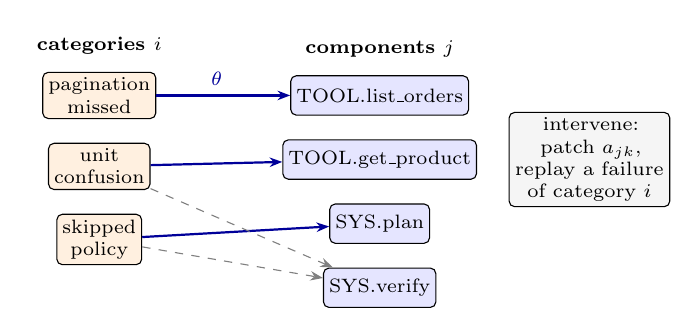
\begin{tikzpicture}[font=\scriptsize, node distance=3mm,
  box/.style={draw, rounded corners=2pt, align=center, inner sep=2pt, minimum height=5mm},
  cat/.style={box, fill=orange!12}, comp/.style={box, fill=blue!10},
  >={Stealth[length=1.6mm]}]
\node[cat] (c1) {pagination\\missed};
\node[cat, below=of c1] (c2) {unit\\confusion};
\node[cat, below=of c2] (c3) {skipped\\policy};
\node[comp, right=17mm of c1] (k1) {TOOL.list\_orders};
\node[comp, below=of k1] (k2) {TOOL.get\_product};
\node[comp, below=of k2] (k3) {SYS.plan};
\node[comp, below=of k3] (k4) {SYS.verify};
\draw[->, thick, blue!60!black] (c1) -- node[above, sloped, pos=.45]{$\theta$} (k1);
\draw[->, thick, blue!60!black] (c2) -- (k2);
\draw[->, thick, blue!60!black] (c3) -- (k3);
\draw[->, dashed, gray] (c2) -- (k4);
\draw[->, dashed, gray] (c3) -- (k4);
\node[above=1mm of c1, font=\scriptsize\bfseries] {categories $i$};
\node[above=1mm of k1, font=\scriptsize\bfseries] {components $j$};
\node[box, right=4mm of k2, text width=19mm, fill=gray!8] (o) {intervene:\\patch $a_{jk}$,\\replay a failure\\of category $i$};
\end{tikzpicture}
\caption{The category--component graph. Solid edges are true causal edges; dashed ones are plausible but wrong attributions (e.g.\ blaming verification for a unit error). Each intervention patches one component and replays one failure.}
\label{fig:graph}
\end{figure}

An agent is built from \emph{components} $j\in\{1,\dots,J\}$: sections of its system prompt, tool descriptions, tool implementations, orchestration settings. Its failures have been grouped into \emph{categories} $i\in\{1,\dots,I\}$ by an LLM, with $f_i$ the share of failures in category $i$. For every cell $(i,j)$ an analyst LLM can propose $K$ candidate patches $a_{ijk}$ that rewrite component $j$ to address category $i$.

\paragraph{Interventions.} An intervention $(i,j,k,\phi)$ samples a failed trajectory labelled $i$, applies patch $a_{ijk}$, and observes a binary outcome at fidelity $\phi$. A \emph{full replay} ($\phi=F$) resumes the episode from the attributed failing step and records whether the task now succeeds. A \emph{single-step check} ($\phi=S$) regenerates only the failing step and asks a judge whether the diagnosed error is gone. They cost $c_F$ and $c_S\ll c_F$.

\paragraph{Edges and patch quality.} We write $e_{ij}\in\{0,1\}$ for whether component $j$ is a cause of category $i$, meaning some change to $j$ repairs a non-trivial fraction of its failures, and $q_{ijk}\in[0,1]$ for the repair probability of patch $k$ when $e_{ij}=1$. This separation matters because a negative replay outcome is ambiguous: either $j$ is the wrong component or $a_{ijk}$ is a bad patch. Testing several patches per cell resolves the ambiguity.

\paragraph{Objective.} After spending at most budget $B$, the method accepts a set of cells $\mathcal{A}$ and, for each, a patch $k^\star_{ij}$. Accepting a true edge repairs a fraction $q_{ijk^\star}$ of category $i$'s failures; accepting a false edge costs a regression $c_{\mathrm{fp}}$, reflecting that unnecessary changes perturb behaviour on tasks that used to succeed \citep{vasudev2026intervention}. We measure
\begin{equation}
\begin{aligned}
G(\mathcal{A}) = {}&\sum_i f_i\Big(1-\!\!\prod_{j\in\mathcal{A}_i^+}\!\!(1-q_{ijk^\star_{ij}})\Big)\\
&- c_{\mathrm{fp}}\,\big|\{(i,j)\in\mathcal{A}:e_{ij}=0\}\big|,
\end{aligned}
\label{eq:gain}
\end{equation}
where $\mathcal{A}_i^+=\{j:(i,j)\in\mathcal{A},\,e_{ij}=1\}$. This is the net failure mass repaired; we report it as a fraction of the oracle value obtained by accepting exactly the true edges with their best patches.


\subsection{\carve{}}
\label{app:cmethod}

\paragraph{Observation model}
For a trajectory labelled $i$ and patch $a_{ijk}$, the probability that a full replay succeeds is
\begin{equation}
p_{ijk} = \begin{cases} \lambda\, q_{ijk} + (1-\lambda)\, b & e_{ij}=1,\\ b & e_{ij}=0,\end{cases}
\end{equation}
where $b$ is the spurious recovery rate (stochastic re-generation sometimes succeeds regardless of the patch) and $\lambda$ is the accuracy of the category labels used to sample trajectories; a mislabelled trajectory is treated as unaffected by the patch. A single-step check returns $z=1$ with probability $s\,p+\epsilon\,(1-p)$, where $s$ and $\epsilon$ are the sensitivity and false-positive rate of the check relative to the full outcome. All four nuisance parameters can be estimated from a small calibration set on which both fidelities and a human audit are run.

\paragraph{Attribution-informed prior}
Let $n_{ij}$ be the number of failures in category $i$ that the analyst attributed to component $j$, and $\hat r$ the analyst's attribution accuracy estimated on a small audited sample. With $d$ the expected number of causal components per category and $\rho=d/J$ the base edge density, we set
\begin{equation}
\pi_{ij} = (1-\hat r)\,\rho + \hat r\,\min\!\big(1,\ d\, n_{ij}/n_i\big),
\label{eq:prior}
\end{equation}
so that an unreliable analyst ($\hat r\to0$) yields the flat prior $\rho$ and a reliable one concentrates mass on the components it names. Eq.~\ref{eq:prior} is a heuristic interpolation, not a calibrated model; with a larger audit, $\pi$ could instead be fitted by logistic regression on audited attributions. Patch quality has prior $q_{ijk}\sim\mathrm{Beta}(\alpha_q,\beta_q)$.

\paragraph{Posterior}
Cells are independent given the data. For each cell we keep the posterior log-odds of $e_{ij}$ and, for each patch, a posterior over $q_{ijk}$ on a fixed grid of $G=101$ points. With $\mathcal{D}_{ijk}$ the outcomes observed for patch $k$,
\begin{equation}
\begin{aligned}
\mathrm{logit}\,P(e_{ij}{=}1\mid\mathcal{D}) ={}& \mathrm{logit}\,\pi_{ij}\\
&+ \textstyle\sum_k \log\big(\bar L^{1}_{ijk}/L^{0}_{ijk}\big),
\end{aligned}
\end{equation}
where $\bar L^{1}_{ijk}=\int P(\mathcal{D}_{ijk}\mid q,e_{ij}{=}1)\,dP(q)$ is the marginal likelihood of patch $k$'s outcomes under a true edge and $L^{0}_{ijk}=P(\mathcal{D}_{ijk}\mid e_{ij}{=}0)$.
Every update multiplies one grid vector by a likelihood vector, so updates and look-aheads are vectorised dot products.

\paragraph{Selecting interventions}
The value of the current decision for cell $(i,j)$, with $P_{ij}$ its edge posterior and $\hat Q_{ij}=\max_k\mathbb{E}[q_{ijk}\mid\mathcal{D}]$, is
\begin{equation}
V_{ij} = \max\big(P_{ij}\,f_i\,\hat Q_{ij} - (1-P_{ij})\,c_{\mathrm{fp}},\ 0\big),
\end{equation}
the expected contribution of the cell to Eq.~\ref{eq:gain} under the Bayes decision (accept iff the first term is positive), treating cells as additive. Eq.~\ref{eq:gain} combines components of one category multiplicatively, so $V_{ij}$ slightly overstates the value of a second cause for an already repaired category; we accept this approximation because it keeps cells independent. For an action $a=(i,j,k,\phi)$ repeated $n$ times, let $V'_{ij}(s)$ be the value after observing $s$ successes. The $n$-step knowledge gradient is
\begin{equation}
\mathrm{KG}_n(a) = \sum_{s=0}^{n} P(s\mid\mathcal{D},a)\,V'_{ij}(s) - V_{ij},
\end{equation}
and \carve{} runs the action maximising
\begin{equation}
\mathrm{score}(a) = \max_{n\in\{1,2,4,8\}} \frac{\mathrm{KG}_n(a)}{n\,c_\phi}.
\label{eq:score}
\end{equation}
Looking ahead several observations matters because a single binary outcome often cannot flip a decision, in which case $\mathrm{KG}_1=0$ even for a valuable cell; maximising over $n$ is the standard remedy \citep{frazier2008kg}. Because cells are independent, only the observed cell's scores change after each outcome, so each step rescores one cell in $O(KG)$ time after an initial pass over all cells.

\paragraph{Decisions and stopping.} At any point the method accepts the cells whose current value is positive and applies, for each, the patch with the highest posterior mean quality. It stops early when no action has a score above a small threshold, i.e.\ when no remaining experiment is expected to be worth its cost.


\subsection{When Do Priors and Cheap Checks Help?}
\label{app:canalysis}

These results analyse an idealised per-cell sequential test, not \carve{}'s full policy; they explain which quantities govern the method's behaviour. We consider a single cell and a single patch with known success probabilities $p_1$ (true edge) and $p_0=b$, under a rule that stops when the posterior log-odds leaves $[-A,A]$, $A=\log\frac{1-\delta}{\delta}$. Let $D_1=\mathrm{KL}(p_1\Vert p_0)$ and $D_0=\mathrm{KL}(p_0\Vert p_1)$ be the expected log-likelihood-ratio drift per observation under each hypothesis. Proofs, which follow Wald's approximations \citep{wald1945sequential}, are in Appendix~\ref{app:cproofs}.

\begin{proposition}[Value of the LLM prior]
\label{prop:cprior}
Let $|\ell|<A$ and neglect overshoot and stopping at the wrong boundary (whose probability is approximately $\delta e^{-\ell}$ for a true edge and $\delta e^{\ell}$ for a false one). A cell with initial log-odds $\ell$ then needs $N_1(\ell)=(A-\ell)/D_1$ observations in expectation if it is a true edge and $N_0(\ell)=(A+\ell)/D_0$ if not. Replacing a flat prior $\ell_\rho$ by LLM-derived log-odds $\ell_{ij}$ saves, in expectation over cells,
\begin{equation}
\Delta = \frac{\rho\,\mathbb{E}[\delta\ell\mid e{=}1]}{D_1} - \frac{(1-\rho)\,\mathbb{E}[\delta\ell\mid e{=}0]}{D_0},
\end{equation}
with $\delta\ell=\ell_{ij}-\ell_\rho$,
observations per cell, which is positive exactly when the prior raises true edges more, relative to their base rate and drift, than it raises false ones.
\end{proposition}

Under Eq.~\ref{eq:prior}, $\ell_{ij}\to\ell_\rho$ as $\hat r\to0$, so $\Delta\to0$: a useless analyst costs nothing beyond the flat prior, whereas trusting its labels outright (LLM-only) makes permanent errors. A miscalibrated analyst can make $\Delta$ negative, but only by an amount linear in the log-odds shift, after which the evidence takes over. Appendix~\ref{app:prop1} compares these predictions with simulated sequential tests.

\begin{proposition}[Cheap checks]
\label{prop:cfid}
Let $D^S_e$ denote the drifts of single-step outcomes, $z\sim\mathrm{Bern}(s\,p_e+\epsilon(1-p_e))$. Under the same approximations, a test using only single-step checks reaches the stopping boundary at lower expected cost than one using only full replays if and only if
\begin{equation}
\frac{c_S}{c_F} < \frac{D^S_e}{D_e},
\end{equation}
where $e$ is the true state of the cell.
\end{proposition}

Since $e$ is unknown, the proposition gives a clear rule only when the cost ratio lies outside the interval spanned by the two critical ratios; inside it, which fidelity is better depends on the posterior, which is what \carve{}'s look-ahead weighs.

With our default parameters ($p_1=0.54$, $b=0.05$, $s=0.85$, $\epsilon=0.15$) the critical ratio is $0.31$ for true edges and $0.44$ for false ones; with a weak check ($s=0.65$, $\epsilon=0.35$) it falls to $0.05$--$0.08$. Section~\ref{app:cfid} tests both predictions.


\subsection{Controlled Experiments}
\label{app:csim}

Real agents do not reveal which component truly caused a failure, so we first evaluate in a testbed where the causal graph is known and the method's model is deliberately misspecified.

\paragraph{Setup}
\paragraph{Testbed.} Each world has $I=12$ categories with Zipfian frequencies, $J=20$ components and $K=3$ patches per cell. Every category has one or two true components and one \emph{decoy} component that wrong attributions prefer, mimicking symptom-level mislabelling. Patch quality is bimodal: with probability 0.3 a patch is bad ($q\sim\mathrm{Beta}(1,9)$), otherwise $q\sim\mathrm{Beta}(6,3)$. A trajectory sampled for category $i$ is mislabelled with probability $1-\lambda=0.2$, in which case it comes from another category (weighted by frequency) and is repaired only if \emph{its own} edge to $j$ exists, unlike the model's flat treatment of mislabelled traces. The analyst attributes 20 failures per category with accuracy $r=0.5$; wrong attributions go to the decoy with probability 0.6. The analyst's accuracy is estimated from an audit of 20 attributions. Costs are $c_F=1$, $c_S=0.1$, $c_{\mathrm{fp}}=0.02$, and $s=0.85$, $\epsilon=0.15$, $b=0.05$. Section~\ref{app:crobust} relaxes the assumptions the generator shares with the model. Full details are in Appendix~\ref{app:sim}.

\paragraph{Baselines.} \emph{LLM-only} accepts, for every category, the most-attributed component and any component holding at least 40\% of the attributions, with the first patch, i.e.\ it acts on an induced taxonomy without verification. \emph{Replay-each} tests attributed hypotheses in order of attribution count with three full replays of the first patch and accepts a hypothesis if at least two succeed, mirroring do-then-verify methods such as DoVer; \emph{Replay-each, 3 patches} gives each hypothesis two replays of each of three patches and accepts if any patch succeeds twice; \emph{Sequential-each} replays each hypothesis, cycling through patches, until \carve{}'s own posterior leaves $[0.05,0.95]$. Untested hypotheses fall back to LLM-only, except for Sequential-each, which uses the Bayes decision. \emph{Thompson sampling} samples $(e,q)$ from the posterior and replays the cell and patch with the largest sampled repair. \emph{Uncertainty sampling} replays the cell with the largest frequency-weighted uncertainty $f_i\min(P_{ij},1-P_{ij})$, cycling through patches, at full fidelity; \emph{Uncertainty + cheap checks} first runs three single-step checks per (cell, patch) and then confirms with full replays. All baselines except LLM-only and the Replay-each variants share \carve{}'s posterior and decision rule, so comparisons among them isolate the selection rule.

\paragraph{Metrics.} Net gain (Eq.~\ref{eq:gain}) as a fraction of the oracle, and edge F1. We report means and standard errors over 50 worlds for the main experiment and 30 for the others; all methods see the same worlds, so differences are paired.

\paragraph{Main results}

\begin{figure*}[t]
\centering
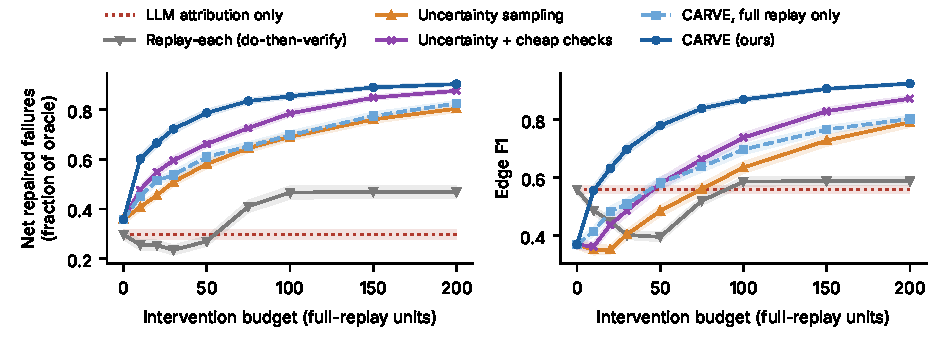
\includegraphics[width=0.85\textwidth]{figures/budget_curves.pdf}
\caption{Net repaired failure mass (left) and edge F1 (right) against intervention budget, 50 worlds, shaded $\pm1$ s.e.}
\label{fig:budget}
\end{figure*}

\begin{table}[t]
\centering
\small
\setlength{\tabcolsep}{3pt}
\resizebox{\columnwidth}{!}{%
\begin{tabular}{lcccc}
\toprule
 & \multicolumn{4}{c}{Budget (full-replay units)}\\
Method & 20 & 50 & 100 & 200 \\
\midrule
\csname @@input\endcsname tables/main.tex 
\bottomrule
\end{tabular}}
\caption{Net gain as a fraction of the oracle (mean $\pm$ s.e., 50 worlds). The lower block ablates \carve{}.}
\label{tab:main}
\end{table}

Figure~\ref{fig:budget} and Table~\ref{tab:main} show that \carve{} is best at every budget. With 50 units it recovers 79\% of the oracle gain; the strongest baseline, uncertainty sampling with the same cheap checks, recovers 66\% and needs about twice the budget (100 units, 78\%) to match it. The gap narrows at large budgets (90\% vs.\ 88\% at 200), as every reasonable method eventually resolves the frequent categories.

\paragraph{Where the gain comes from.} Two comparisons separate the selection rule from the cheap checks. With full replays only, \carve{} beats uncertainty sampling by 1--6 points (e.g.\ 0.609 vs.\ 0.581 at budget 50): the knowledge-gradient rule alone helps only modestly. Given cheap checks, its advantage grows to 7--13 points (0.787 vs.\ 0.662 at 50), because it decides per action whether a check is informative enough for its price and stops checking a cell once checks can no longer change the decision, whereas a fixed check-then-confirm schedule wastes checks on resolved cells. Most of \carve{}'s advantage is therefore in \emph{how it uses} cheap checks, which also makes their calibration critical (\S\ref{app:crobust}).

\paragraph{Verification baselines.} LLM-only is stuck at 30\% because it accepts decoys and bad first patches. Replay-each is initially \emph{worse} than not verifying: with $p_1\approx0.54$, requiring two successes in three replays rejects about 44\% of true edges even when the patch is good, and its fixed per-hypothesis cost exhausts small budgets on frequent but already-certain hypotheses. Testing three patches (61\% at 200) or stopping adaptively (81\% at 200) helps, but both remain well below \carve{} at small budgets (32\% and 52\% at 50). Thompson sampling spends most replays on cells it already believes in and reaches only 63\% at 200.

\paragraph{Ablations.} Removing single-step checks costs 15--18 points at small budgets. Restricting the look-ahead to one observation is below the full method at every budget and plateaus at 73\%, because many cells cannot be flipped by a single outcome and are never revisited. A flat prior costs 32 points at budget 20 and still 10 points at 200. With one patch per cell the method plateaus at 69\%: it cannot tell a wrong component from a bad patch and rejects true edges for good. Dropping the label-noise term makes no difference at the default label accuracy $\lambda=0.8$ (it is even slightly better at large budgets, 0.922 vs.\ 0.902 at 200), but it matters when labels are worse (\S\ref{app:crobust}).

\paragraph{When does the LLM prior help?}

\begin{figure}[t]
\centering
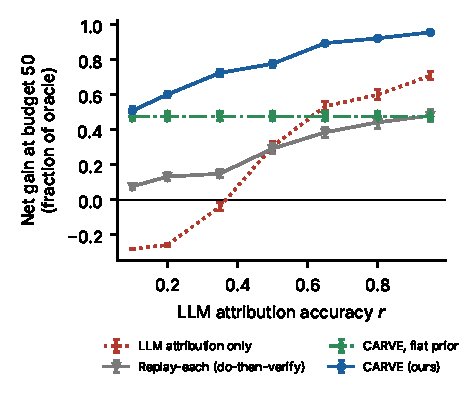
\includegraphics[width=\columnwidth]{figures/prior_sweep.pdf}
\caption{Net gain at budget 50 as the analyst's attribution accuracy $r$ varies (30 worlds, $\pm1$ s.e.).}
\label{fig:prior}
\end{figure}

Figure~\ref{fig:prior} varies the analyst's accuracy $r$. As Proposition~\ref{prop:cprior} suggests, \carve{} improves monotonically with $r$ and is never below the flat-prior variant: at $r=0.1$ it scores $0.51\pm0.02$ against $0.48\pm0.03$. The prior is not exactly flat there (the decoy still receives about twice the base rate), but its shifts are small, so evidence quickly dominates. Acting on attributions directly is harmful below $r\approx0.35$, where LLM-only has a \emph{negative} net gain (regressions outweigh repairs), and even at $r=0.95$ it reaches only 71\% of the oracle against 96\% for \carve{}, since it cannot detect bad patches. Replay-each improves with $r$ and only matches the flat-prior variant of \carve{} at $r=0.95$ ($0.48$ vs.\ $0.48$).

\paragraph{When do cheap checks help?}
\label{app:cfid}

Figure~\ref{fig:fid} (Appendix~\ref{app:extra}) is qualitatively consistent with Proposition~\ref{prop:cfid}. With the default check, the benefit of cheap checks shrinks as their cost grows and vanishes between 0.35 and 0.5 ($0.64\pm0.02$ vs.\ $0.61\pm0.03$ at 0.35, overlapping; $0.59$ vs.\ $0.61$ at 0.5), in line with the predicted critical ratios of 0.31 and 0.44. At cost 0.1, a check of quality $s-\epsilon=0.5$ (critical ratio 0.14--0.22) still helps, while one of quality 0.3 (critical ratio 0.05--0.08) brings no gain. At cost 0.5 \carve{} is slightly below its full-replay-only variant although its action set contains every full-replay action, which shows that the greedy rule is not exactly cost-optimal when the two fidelities are nearly equally efficient.

\paragraph{Robustness}
\label{app:crobust}

\begin{table}[t]
\centering
\small
\setlength{\tabcolsep}{3pt}
\resizebox{\columnwidth}{!}{%
\begin{tabular}{lcc}
\toprule
Condition (budget 50) & Unc.\ + checks & \carve{} \\
\midrule
\csname @@input\endcsname tables/stress.tex 
\bottomrule
\end{tabular}}
\caption{Violations of the model's assumptions (30 worlds). The judge-fooled row is the one setting where \carve{} loses.}
\label{tab:stress}
\end{table}

The generator shares several assumptions with the model: check errors depend only on the full outcome, cells are independent, the analyst's accuracy is estimated without bias, and the regression cost is small. Table~\ref{tab:stress} and Appendix~\ref{app:extra} relax each in turn.

\paragraph{Worse labels.} With label accuracy $\lambda=0.5$ both methods lose ground, and the label-noise term now matters: \carve{} scores 0.688, against 0.588 without the term and 0.513 for the baseline.

\paragraph{Biased analyst audit.} If the audit overstates the analyst's accuracy by 0.3, \carve{} actually improves (0.857), because a stronger prior concentrates the budget and the evidence corrects the decoys. Understating it by 0.3 costs 12 points (0.653), still above the baseline. Under-trusting a decent analyst is thus the more costly error in this testbed.

\paragraph{Regression cost.} Raising $c_{\mathrm{fp}}$ from 0.005 to 0.1 leaves \carve{} between 0.78 and 0.82, while LLM-only falls from 0.39 to $-0.13$: the more costly a wrong change, the more verification is worth.

\paragraph{Joint causes.} When 30\% of categories need two components changed together (a single patch then repairs only a fifth as often), violating cell independence, \carve{} drops from 0.787 to 0.661 at budget 50 but stays ahead of uncertainty sampling with checks (0.558; Table~\ref{tab:joint}).

\paragraph{Correlated check errors.} The one setting where \carve{} loses is when the single-step judge is fooled by plausible-looking bad patches (false-positive rate 0.6 for patches with $q<0.3$). \carve{} then trusts checks that systematically pass bad patches and falls to 0.377, below every method that relies on full replays (0.58--0.61). Modelling the dependence (a quality-dependent false-positive rate in the likelihood) restores it to 0.584, on par with full replays, at a cost of 9 points when the judge is not fooled (0.684 vs.\ 0.776). Whether real judges behave this way is therefore the most important quantity to measure before relying on cheap checks.

\paragraph{Nuisance parameters and scale.} Misspecifying $b$, $\lambda$ or the patch-quality prior changes the result by at most 5 points (Table~\ref{tab:misspec}, Appendix~\ref{app:extra}); misstating the check's sensitivity and false-positive rate costs 6--14 points. On a larger graph ($I=20$, $J=50$; Table~\ref{tab:scale}) the gap widens: at budget 50 \carve{} reaches 78\% of the oracle against 60\% for uncertainty sampling with checks.

\paragraph{Inside a self-improvement loop}

\begin{figure}[t]
\centering
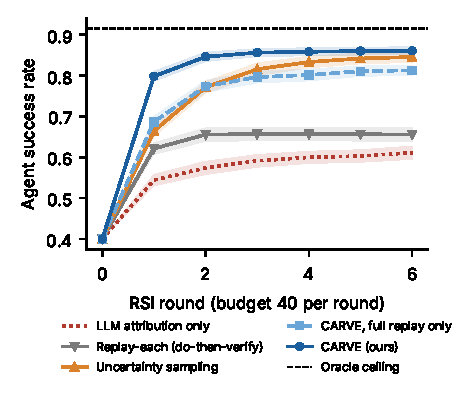
\includegraphics[width=\columnwidth]{figures/rsi.pdf}
\caption{Agent success over six rounds of attribute--verify--patch, with a budget of 40 units per round (30 worlds, $\pm1$ s.e.).}
\label{fig:rsi}
\end{figure}

Finally we embed each method in a loop. The agent starts at 40\% success. In each round the analyst attributes 240 new failures, sampled in proportion to the current failure distribution; the method spends 40 units; accepted patches are applied, which repairs failures (true edges) or adds a regression of $c_{\mathrm{fp}}$ times the current failure mass (false edges); and the failure distribution is recomputed, so priorities shift towards categories that remain. Posteriors carry over between rounds.

Figure~\ref{fig:rsi} shows that \carve{} reaches 80\% success after one round and 85\% after two, close to its plateau of 86\% (the oracle ceiling is 91.5\%). Uncertainty sampling with checks needs four rounds to reach 84\% and ends at 85\%; without checks it needs six. LLM-only and Replay-each plateau at 61\% and 66\%: once their accepted false edges and rejected true edges are fixed in place, new attributions do not correct them.


\subsection{Proofs for \carve{}'s propositions}
\label{app:cproofs}

\paragraph{Proposition~\ref{prop:cprior}.} Let $L_t=\ell+\sum_{u\le t}\log\frac{P(o_u\mid e=1)}{P(o_u\mid e=0)}$ be the posterior log-odds after $t$ observations. Under $e=1$, the increments are i.i.d.\ with mean $D_1=\mathrm{KL}(p_1\Vert p_0)>0$. The rule stops at $N=\inf\{t: L_t\notin(-A,A)\}$. By Wald's identity, $\mathbb{E}_1[L_N-\ell]=D_1\,\mathbb{E}_1[N]$. Wald's approximations give $P_1(L_N\le -A)\approx e^{-(A+\ell)}\approx\delta e^{-\ell}$ and $P_0(L_N\ge A)\approx\delta e^{\ell}$. Neglecting overshoot and this probability (which requires $\delta e^{|\ell|}\ll1$), $L_N=A$, hence $\mathbb{E}_1[N]=(A-\ell)/D_1$; if $\ell\ge A$ no observation is taken, which is why we assume $|\ell|<A$. Symmetrically, under $e=0$ the drift is $-D_0$ and $\mathbb{E}_0[N]=(A+\ell)/D_0$. Taking the difference between $\ell_\rho$ and $\ell_{ij}$ and averaging over cells with $P(e{=}1)=\rho$ gives $\Delta$. When the patch quality $q$ is unknown, outcomes are exchangeable rather than i.i.d.\ under the marginal likelihood, and Wald's identity does not apply directly; conditioning on $q$ recovers the result with $D_1=D_1(q)$, which approaches zero for a bad patch. This is the formal reason a single bad patch can stall verification and why \carve{} keeps several patches per cell.

\paragraph{Proposition~\ref{prop:cfid}.} By the same argument a single-step test needs $(A\mp\ell)/D^S_e$ observations at cost $c_S$ each, and a full-replay test needs $(A\mp\ell)/D_e$ at cost $c_F$. The single-step test is cheaper iff $c_S/D^S_e<c_F/D_e$. Since the single-step outcome is a garbling of the full outcome, the data-processing inequality gives $D^S_e\le D_e$, so the critical ratio is at most one.

\subsection{Simulation Details}
\label{app:sim}

Category frequencies are $f_i\propto 1/i$. For each category the number of true components is uniform on $\{1,2\}$ and the decoy is a further distinct component. The audit estimate $\hat r$ is a binomial proportion from 20 audited attributions. The prior uses $d=1.5$. The model's grid has 101 points; look-ahead horizons are $\{1,2,4,8\}$; the stopping threshold is $10^{-6}$. Replay-each uses three replays and accepts with at least two successes. Uncertainty sampling switches to an untried patch once the current patch has three full observations. In the loop experiment, 240 attributions per round are allocated to categories by a multinomial draw with the current failure distribution. All randomness is seeded; the code reproduces every number in this paper with \texttt{python -m sim.experiments all}.

\subsection{Checking Proposition~\ref{prop:cprior}}
\label{app:prop1}

Table~\ref{tab:prop1} compares the predicted expected number of observations with simulated sequential tests ($p_1=0.543$, $p_0=0.05$, $\delta=0.02$, 4000 runs per row). The predictions capture the direction and approximate size of the effect of the initial log-odds; they are least accurate when $|\ell|$ is large, where overshoot and wrong-boundary exits (last column) are no longer negligible.

\begin{table}[h]
\centering
\small
\begin{tabular}{rcccc}
\toprule
$\ell$ & $e$ & predicted $N$ & simulated $N$ & wrong exit \\
\midrule
\csname @@input\endcsname tables/prop1.tex 
\bottomrule
\end{tabular}
\caption{Proposition~\ref{prop:cprior}: predicted vs.\ simulated observations to a decision.}
\label{tab:prop1}
\end{table}

\subsection{Additional Results}
\label{app:extra}
\begin{figure}[t]
\centering
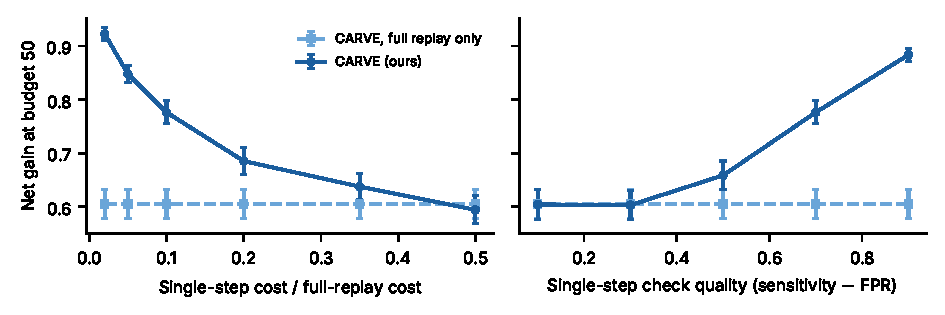
\includegraphics[width=\columnwidth]{figures/fidelity.pdf}
\caption{Effect of the single-step check's cost (left, quality fixed at $s{=}0.85$, $\epsilon{=}0.15$) and quality (right, cost fixed at 0.1) on net gain at budget 50.}
\label{fig:fid}
\end{figure}

\begin{table}[h]
\centering
\small
\setlength{\tabcolsep}{3pt}
\resizebox{\columnwidth}{!}{%
\begin{tabular}{lccc}
\toprule
Method & 50 & 100 & 300 \\
\midrule
\csname @@input\endcsname tables/scale.tex 
\bottomrule
\end{tabular}}
\caption{Net gain on a larger graph ($I{=}20$, $J{=}50$), 20 worlds.}
\label{tab:scale}
\end{table}

\begin{table}[h]
\centering
\small
\setlength{\tabcolsep}{3pt}
\resizebox{\columnwidth}{!}{%
\begin{tabular}{lcccc}
\toprule
Method & 20 & 50 & 100 & 200 \\
\midrule
\csname @@input\endcsname tables/joint.tex 
\bottomrule
\end{tabular}}
\caption{Net gain when 30\% of categories need two components changed together (30 worlds).}
\label{tab:joint}
\end{table}

\begin{table}[h]
\centering
\small
\begin{tabular}{lc}
\toprule
Model assumption (true value) & Net gain \\
\midrule
All nuisance parameters as in the generator & 0.776\,{\scriptsize$\pm$0.021}\\
Spurious rate $b$: 0.01 (0.05) & 0.811\,{\scriptsize$\pm$0.012}\\
Spurious rate $b$: 0.15 (0.05) & 0.826\,{\scriptsize$\pm$0.016}\\
Label accuracy $\lambda$: 1.0 (0.8) & 0.768\,{\scriptsize$\pm$0.022}\\
Label accuracy $\lambda$: 0.6 (0.8) & 0.794\,{\scriptsize$\pm$0.017}\\
Check $s/\epsilon$: .95/.05 (.85/.15) & 0.717\,{\scriptsize$\pm$0.016}\\
Check $s/\epsilon$: .70/.30 (.85/.15) & 0.636\,{\scriptsize$\pm$0.021}\\
Patch prior $\mathrm{Beta}(1,1)$ ($\mathrm{Beta}(2,2)$) & 0.811\,{\scriptsize$\pm$0.015}\\
Patch prior $\mathrm{Beta}(5,2)$ ($\mathrm{Beta}(2,2)$) & 0.777\,{\scriptsize$\pm$0.020}\\
\bottomrule
\end{tabular}
\caption{\carve{} with misspecified nuisance parameters, budget 50, 30 worlds. Several ``wrong'' values do slightly better than the generator's, a reminder that the model is misspecified in other ways too.}
\label{tab:misspec}
\end{table}


\bibliography{references}

\end{document}
